\documentclass[12pt,a4paper]{report}

% Packages
\usepackage{amsmath}
\usepackage{amsthm}
\usepackage{amssymb}
\newtheorem{definition}{Definition}
\usepackage[utf8]{inputenc}
\usepackage[T1]{fontenc}
\usepackage{biblatex} %Imports biblatex Package
\addbibresource{references.bib}
\usepackage{graphicx}
\graphicspath{ {images/} }
\usepackage[rightcaption]{sidecap}
\usepackage{caption}
\captionsetup{font=small}
\usepackage{booktabs}
\usepackage{setspace}
\usepackage{geometry}
\usepackage{hyperref}
\usepackage{titlesec}
\usepackage{lipsum}
\usepackage{xcolor}
\usepackage{algorithm}
\usepackage{algpseudocode}
\usepackage{subcaption}
\usepackage{caption}
\usepackage{float}

% Set margins
\geometry{
    left=1.5in,
    right=1in,
    top=1in,
    bottom=1in,
    headheight=14.5pt
}

% Title page formatting
\titleformat{\chapter}[display]
  {\normalfont\huge\bfseries}{\chaptertitlename\ \thechapter}{20pt}{\Huge}

% Begin document
\begin{document}

\pagenumbering{roman}

% Title page
\begin{titlepage}
    \centering
    
\includegraphics[width=0.4\textwidth]{cmi-header.png}\par\vspace{1cm}
    {\scshape\Large Master's Thesis\par}
    \vspace{1.5cm}
    {\huge\bfseries State Space Models: An Efficient Alternative to Attention\par}
    \vspace{2cm}
    {\Large Sampad Kumar Kar\par}
    \vspace{0.5cm}
    {\Large Supervised by Prof. Pranabendu Misra\par}

    \vspace{2cm}

    \begin{figure}[h]
        \centering
        \includegraphics[scale=0.6]{cover/cover_pic.png}
    \end{figure}
    
    \vfill

    % Bottom of the page
    {\large \today\par}
\end{titlepage}

% Abstract
\chapter*{Abstract}
The Transformer architecture, with its core self-attention mechanism, has revolutionised deep learning, achieving state-of-the-art results across various tasks. However, the quadratic scaling of attention with sequence length presents a significant bottleneck for handling long sequences. This has driven the exploration of alternative sequence modelling paradigms, with state space models (SSMs) emerging as a promising contender. This survey delves into the recent advancements in SSMs, focusing on their theoretical foundations, key architectures, and empirical performance. We discuss prominent SSM variants, including S4, Mamba, Linear Recurrent Units (LRUs) and Griffin, highlighting their unique strengths in addressing challenges like computational efficiency and capturing long-range dependencies. We also present experimentals on toy datasets, demonstrating their performance in text, image, and audio generation using tiny LLMs.

% Acknowledgments
% \chapter*{Acknowledgments}
% \lipsum[2]

% Table of Contents
\tableofcontents

% Chapters
\chapter*{Introduction}
\pagenumbering{arabic}

Recurrent Neural Networks (RNNs) have historically been the dominant paradigm for sequence modelling, achieving SoT results in tasks such as Machine Translation, Text Generation, and Speech Recognition. RNNs excel at capturing sequential information by iteratively updating a hidden state based on the current input and the previous state. However, RNNs are inherently limited in their ability to handle long-range dependencies (LRDs), as information from the distant past can be lost due to the vanishing gradient problem. This restriction led to the development of Long Short-Term Memory (LSTM) networks, which introduced gating mechanisms to selectively remember or forget information, mitigating some of the drawbacks of traditional RNNs.

Despite these advancements, RNNs and LSTMs still face challenges in capturing LRDs effectively and efficiently. Training these models is often slow due to their sequential nature, and they can struggle to generalise when the length of the input sequence varies.

\medskip

The emergence of Transformers \cite{transformers} as an alternative sequence modelling paradigm has significantly shifted the landscape. Transformers, with their core self-attention mechanism, allow each token to interact with every other token in the input sequence, enabling them to capture LRDs effectively. This has led to a surge in performance across various tasks, making Transformers the dominant paradigm in NLP and other sequence-to-sequence tasks.

However, Transformers are not without their shortcomings. The quadratic complexity of their self-attention mechanism, scaling as $\mathcal{O}(n^2)$ with sequence length $n$, poses a significant computational bottleneck, especially when dealing with long sequences in domains like genomics and high-resolution image analysis. Moreover, Transformers also struggle in the Long Range Arena (LRA) benchmark, a suite of challenging tasks designed to test models' ability to reason over very long sequences. This suggests that Transformers, despite their overall strength, might not be the ideal solution for all sequence modelling tasks, particularly those demanding efficient processing of long sequences.

\medskip

State Space Models (SSMs) have emerged as a compelling alternative to Transformers, offering key efficiency advantages. SSMs, inspired by classical models from control theory and signal processing, compress input data into a fixed-size latent state during sequence generation. This static memory allocation enables SSMs to process long sequences efficiently without the quadratic complexity of attention. Furthermore, SSMs can be computationally advantageous during inference, exhibiting faster processing compared to Transformers.

\medskip

This survey delves into the recent advancements in SSMs, focusing on their theoretical foundations, key architectures, and empirical performance. We examine prominent SSM variants, including S4 \cite{s4}, Mamba \cite{mamba}, Linear Recurrent Units (LRUs) \cite{lru}, and Griffin \cite{hawkgriffin}, highlighting their unique strengths in addressing challenges like computational efficiency and capturing LRDs. We also present experimental results on toy datasets, demonstrating their performance in text, image, and audio generation using tiny LLMs.

\medskip

We organised the thesis into the chapters as follows:
\begin{itemize}
    \item \textbf{Chapter 1} outlines the framework for deep sequence modelling, outlining the key challenges in this domain, including the LRA benchmark.
    \item \textbf{Chapter 2} provides a background on Transformers and the Attention mechanism and its limitations.
    \item \textbf{Chapter 3} introduces the SSM framework, discussing its conceptual foundation and fundamental principles. Then it delves into the S4 architecture, a prominent SSM variant, exploring its unique characteristics and how it overcomes the computational limitations of previous SSM models, including the core mechanics of S4.
    \item \textbf{Chapter 4} focuses on Mamba, a more recent SSM architecture, emphasising its selective state space and its ability to efficiently process long sequences.
    \item \textbf{Chapter 5} introduces LRUs and their theoretical universality. We discuss how LRUs can be designed to achieve comparable performance to SSMs with minimal architectural changes.
    \item \textbf{Chapter 6} examines Hawk and Griffin architecture, which combines the strengths of LRUs and local attention to achieve even higher performance and efficiency.
    \item \textbf{Chapter 7} presents some experimentals, showcasing the capabilities of SSMs on some toy datasets.
\end{itemize}

\chapter{Introduction to Deep Sequence Modelling}

\section{Deep Sequence Models}
Deep learning methods have made significant advances in machine learning, achieving widespread success across scientific and industrial applications. A core class of models are sequence models, which are parameterised mappings operating on arbitrary sequences of inputs. These can be applied to a wide variety of complex sequential tasks such as:
\begin{itemize}
    \item \textbf{Language Modelling}: The input is a sequence of tokens representing words, and the output is a probability distribution over the next word in the sequence.
    \item \textbf{Machine Translation}: The input is a sequence of tokens representing a sentence in one language, and the output is a sequence of tokens representing the translation in another language.
    \item \textbf{Speech Recognition}: The input is a sequence of audio samples representing speech, and the output is a sequence of tokens representing the transcribed text.
    \item \textbf{Image Captioning}: The input is a sequence of pixels representing an image, and the output is a sequence of tokens representing a textual description of the image.
    \item \textbf{Time Series Forecasting}: The input is a sequence of historical data points, and the output is a prediction of future data points.
\end{itemize}

\begin{SCfigure}[1][ht]
    {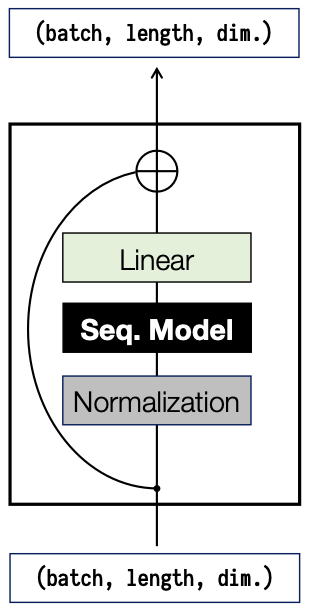
\includegraphics[width=5cm, height=8cm]{C1.1_Deep_Sequence_Models_GenArch.png}}
    \caption{A deep sequence model is a neural network architecture built around a core sequence transformation such as convolutions, attention, or recurrence, and comprising additional components such as normalisation layers, linear layers, and residual connections. This boxed architecture block is usually composed repeatedly into a deep neural network.}
    \label{deep-sequence-arch}
\end{SCfigure}

\begin{definition}
    A \textbf{Sequence Model} is a parameterised map on sequences denoted as $y = f_\theta(x)$ where:
    \begin{itemize}
        \item \textbf{Inputs} ($x$): A sequence of length $L$ of feature vectors in $\mathbb{R}^D$, i.e., $x \in \mathbb{R}^{L \times D}$. Here, $L$ represents the sequence length and $D$ represents the number of features or channels. Each element $x_k \in \mathbb{R}^D$ corresponds to the feature vector at position $k$ in the sequence.
        \item \textbf{Outputs} ($y$): A sequence of length $L$ of feature vectors, i.e., $y \in \mathbb{R}^{L \times D'}$. The output dimension $D'$. Each element $y_k \in \mathbb{R}^{D'}$ corresponds to the output feature vector at position $k$.
        \item \textbf{Parameters} ($\theta$): A collection of parameters learned through gradient descent.
    \end{itemize}
\end{definition}

We can define different deep sequence models by replacing the core sequence model layer (which maps $\mathbb{R}^{B \times L \times D}$ to $\mathbb{R}^{B \times L \times D}$) \footnote{We are interested in cases where $D = D'$} with various sequence modelling mechanisms. Here, $B$ represents the batch size. This framework allows us to explore different architectures and their strengths.

\begin{itemize}
    \item \textbf{Attention} \cite{transformers}: This is the core mechanism of Transformers, which allows for global interactions between all elements in a sequence. The complexity of attention scales quadratically with sequence length, making it inefficient for long sequences.
    \item \textbf{S4} \cite{s4}: The S4 model utilises a structured state space model (SSM) that leverages linear recurrences for efficient computations.
    \item \textbf{Mamba} \cite{mamba}: The Mamba model also utilises SSMs but incorporates a selection mechanism. This mechanism enables the model to selectively propagate or forget information based on the current input token, resulting in more effective modelling.
    \item \textbf{Linear Recurrent Units (LRUs)} \cite{lru}: LRUs achieve comparable performance to SSMs by carefully designing deep RNNs using linear recurrences, specific parameterisations, and normalisation.
    \item \textbf{Hawk and Griffin} \cite{hawkgriffin}: These architectures combine the strengths of LRUs and local attention to achieve even higher performance and efficiency.
\end{itemize}

Deep sequence models also face several challenges:
\begin{itemize}
    \item \textbf{General-Purpose Capabilities}: Developing sequence models that can perform effectively across various domains and capabilities requires addressing the specific strengths and weaknesses of different model families.
    \item \textbf{Computational Efficiency}: Ensuring efficient computation of the sequence-to-sequence mapping is crucial, especially for long sequences and online/autoregressive settings.
    \item \textbf{Long-Range Dependencies}: Modelling complex interactions within long sequences is a key challenge. Existing approaches often struggle with capturing LRDs effectively and efficiently.
\end{itemize}

In order to test these models over LRDs, we introduce the \textbf{Long Range Arena} (LRA) Benchmark \cite{lra}.

\section{Long Range Arena}
The LRA Benchmark, introduced by Tay et al. \cite{lra} is a suite of challenging tasks designed to test models' ability to reason over very long sequences. The benchmark consists of a diverse set of tasks, including:
\begin{itemize}
    \item \textbf{Long ListOps}: This task evaluates the model's ability to perform nested mathematical operations on a sequence of up to 2K tokens. It tests the model's hierarchical reasoning capabilities over long contexts.
    \item \textbf{Byte-level Text Classification}: This task involves classifying text into categories at the byte/character level, challenging models to compose and aggregate information over longer sequences. The IMDb reviews dataset is used for this task, with a fixed maximum length of 4K tokens.
    \item \textbf{Byte-level Document Retrieval}: This task tests the model's ability to encode and store compressed representations of long sequences suitable for similarity-based matching. The ACL Anthology Network dataset is used, requiring the model to determine whether two papers have a citation link.
    \item \textbf{Image Classification on Sequences of Pixels}: The input is a sequence of pixels representing a flattened image, forcing the model to learn 2D spatial relations between pixels while presented with a 1D sequence. The CIFAR-10 dataset is used for this task.
\end{itemize}

Apart from these tasks, the Pathfinder and PathX tasks are particularly interesting due to their emphasis on long-range spatial dependency.

\subsection{Pathfinder and PathX}

\begin{figure}[ht]
    \centerline{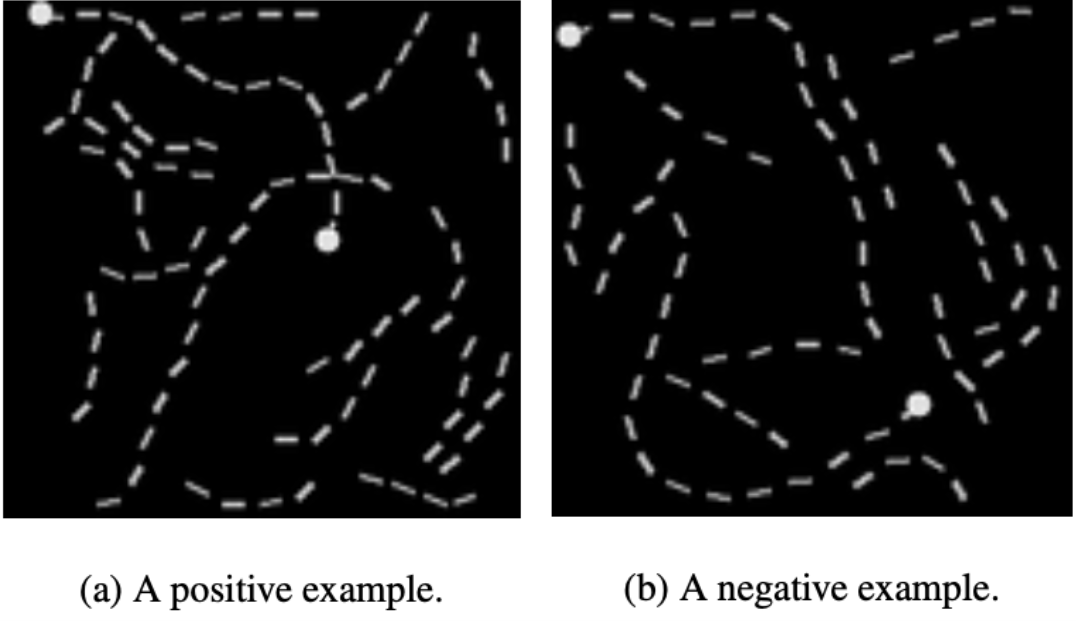
\includegraphics[scale=0.5]{C1.2_PathFinder_Tasks.png}}
    \caption{Samples of Pathfinder task.}
    \label{pathfinder-task}
\end{figure}

Pathfinder (and its more challenging variant, PathX) was designed to probe the ability of models to learn long-range spatial dependencies. It presents a synthetic visual task where a model needs to decide whether two points (represented as circles) are connected by a path consisting of dashes. The task is designed to be difficult due to the presence of distractor paths and variations in the path shape, requiring the model to reason over the entire image to identify the target contour and trace it from one end to the other.

\begin{itemize}
    \item \textbf{Pathfinder}: The input images are $32 \times 32$ pixels, resulting in a sequence length of $1024$.
    \item \textbf{PathX}: This variant increases the difficulty significantly by scaling up the image resolution to $128 \times 128$, resulting in a sequence length of $16384$.
\end{itemize}

At the time LRA was proposed, no model could successfully solve the PathX task, with most models achieving no better than random guessing. This highlights the computational and conceptual challenges posed by models in reasoning over such long sequences. \textbf{S4 \cite{s4} was the first model to successfully crack the PathX task}, achieving remarkable performance on the LRA benchmark. This breakthrough underscored the potential of SSMs as a powerful alternative to Transformers \cite{transformers}, particularly in handling long sequences and challenging LRD tasks.

\chapter{Transformers and the Attention Mechanism}

\section{Transformers and Attention}

The Transformer architecture, introduced by Vaswani et al. \cite{transformers} is based on an encoder-decoder structure, typically using a stacked architecture of encoder and decoder blocks.

\subsection{Encoder Block}
An encoder block generally comprises the following components, sequentially applied to the input sequence:
\begin{itemize}
    \item \textbf{Multi-Head Self-Attention Layer}: This layer computes global interactions between all tokens within a sequence, capturing long-range dependencies.
    \item \textbf{Feedforward Network}: This layer performs position-wise transformations on the output of the attention layer, enhancing the representation of each token.
    \item \textbf{Residual Connections}: These connections skip layers, preventing vanishing gradients and allowing information flow from earlier layers to later layers.
    \item \textbf{Layer Normalisation}: This normalisation technique helps stabilise training and improve generalisation by scaling the output of each layer.
\end{itemize}

\subsection{Decoder Block}
Similar to the encoder block, the decoder block typically includes:
\begin{itemize}
    \item \textbf{Masked Multi-Head Self-Attention Layer}: This layer is masked to ensure that the decoder attends only to previously generated tokens, maintaining the autoregressive property.
    \item \textbf{Encoder-Decoder Attention Layer}: This layer allows the decoder to attend to the output of the encoder, incorporating information from the input sequence.
    \item \textbf{Feedforward Network}: This layer performs position-wise transformations on the output of the attention layers, similar to the encoder block.
    \item \textbf{Residual Connections}: These connections skip layers, preventing vanishing gradients and allowing information flow from earlier layers to later layers.
    \item \textbf{Layer Normalisation}: This normalisation technique helps stabilise training and improve generalisation by scaling the output of each layer.
\end{itemize}

The output of the final decoder layer is then typically passed through a linear projection and a softmax layer to generate a probability distribution over the vocabulary, which is used for tasks such as text generation.

\section{Attention Mechanism}
The attention mechanism \cite{transformers} is the core of the Transformer architecture. It allows the model to dynamically focus on specific parts of the input sequence, effectively weighting the importance of different tokens when generating the output. The most common form is self-attention, where the model attends to itself.

\subsection{Self-Attention}
Let's define self-attention mathematically:
\begin{itemize}
    \item \textbf{Input sequence}: $x = (x_1, x_2, ..., x_n) \in \mathbb{R}^{n \times d}$ represents a sequence of $n$ tokens, where each token $x_i \in \mathbb{R}^d$ is a $d$-dimensional vector.
    \item \textbf{Query, Key, and Value Matrices}: The input sequence is projected into three matrices:
    \begin{itemize}
        \item \textbf{Query Matrix}: $Q \in \mathbb{R}^{n \times d_k}$ is a projection of the input sequence, where $d_k$ is the key dimension.
        \item \textbf{Key Matrix}: $K \in \mathbb{R}^{n \times d_k}$ is another projection of the input sequence, where $d_k$ is the key dimension.
        \item \textbf{Value Matrix}: $V \in \mathbb{R}^{n \times d_v}$ is a projection of the input sequence, where $d_v$ is the value dimension.
    \end{itemize}
    \item \textbf{Attention Weights}: The attention weights are computed by taking the dot product of the query matrix with the key matrix, followed by a softmax normalization:
    \begin{itemize}
        \item \textbf{Similarity Matrix}: $S = QK^T \in \mathbb{R}^{n \times n}$
        \item \textbf{Attention Weights}: $A = softmax(S) \in \mathbb{R}^{n \times n}$
    \end{itemize}
    \item \textbf{Output}: Finally, the attention output is computed by multiplying the attention weights with the value matrix:
    \begin{itemize}
        \item \textbf{Attention Output}: $O = AV \in \mathbb{R}^{n \times d_v}$.
    \end{itemize}
\end{itemize}

This process allows the model to dynamically attend to specific tokens in the input sequence, effectively weighing the contribution of each token to the output.

\subsection{Scaled Dot-Product Attention}
A common implementation of the attention mechanism is Scaled Dot-Product Attention \cite{transformers}. It introduces a scaling factor to the dot product, dividing by $\sqrt{d_k}$, to prevent the dot products from becoming too large and causing numerical instability in the softmax function. This results in the following equation:
\[Attention(Q,K,V) = softmax( \frac{QK^T}{\sqrt{d_k}} )V\]

\subsection{Multi-Head Attention}
To further enhance the expressivity of the attention mechanism, the Multi-Head Attention \cite{transformers} architecture is used. It performs multiple attention calculations in parallel, with each head focusing on different aspects of the input. The outputs of each head are then concatenated and projected to form the final attention output. This is commonly defined with $h$ heads as follows:
\[MultiHead(Q,K,V) = Concat(head_1, ..., head_h)W^O\]
where $head_i = Attention(QW^Q_i, KW^K_i, VW^V_i)$, with the learnable projection matrices $W^Q_i \in \mathbb{R}^{d_{model} \times d_k}, W^K_i \in \mathbb{R}^{d_{model} \times d_k}, W^V_i \in \mathbb{R}^{d_{model} \times d_v}$, and $W^O \in \mathbb{R}^{hd_v \times d_{model}}$.


\section{Limitations of Attention}
While Transformers with their attention mechanism have achieved impressive performance they still have a few limitations:
\begin{itemize}
    \item \textbf{Quadratic Complexity}: The self-attention in Transformers requires computing a similarity matrix between all token pairs in the input sequence, resulting in a complexity of $\mathcal{O}(n^2)$. This means the computational cost and memory requirements grow quadratically with the sequence length $n$. This makes it computationally expensive to process long sequences, especially in domains like genomics and high-resolution image analysis.
    \item \textbf{Inference Speed}: Inference speed of Transformers still scales linearly with the sequence length. This is because the KV cache \cite{mqa}, storing key and value vectors for each token, grows linearly with the sequence length. This can make inference slow and impractical for real-time applications or those requiring the processing of very long sequences.
    \item \textbf{Long Range Arena Benchmark}: Until very recently, the computational limitations of Transformers prevented them from successfully tackling the challenging \textbf{PathX} task in the LRA benchmark \cite{lra}. This task, with a sequence length of $16384$, necessitates capturing long-range spatial dependencies, highlighting the difficulty faced by Transformers in reasoning over very long sequences. Only with the advancement in GPUs and compute power did Transformers start to achieve decent results on this benchmark.
\end{itemize}

These limitations have motivated researchers to explore alternative sequence modelling paradigms, with SSMs emerging as a promising contender that can address these challenges.

\chapter{SSMs: Foundations and the S4 Architecture}

The Transformer architecture, with its core self-attention mechanism, has revolutionized deep learning, achieving state-of-the-art results across a wide range of tasks. However, as discussed in \textbf{Section 2.3}, the quadratic scaling of attention with sequence length poses a significant bottleneck for handling long sequences. This has driven the exploration of alternative sequence modeling paradigms, with SSMs emerging as a promising contender.

\medskip

SSMs, inspired by classical models from control theory and signal processing, offer a continuous-time framework for capturing the dynamics of sequences. The core idea is to represent sequential data through a latent state that evolves over time, allowing for efficient representation and processing of long sequences.

\medskip

The next few chapters dive into the recent advancements in SSMs, focusing on their theoretical foundations and their practical implementation. We start by exploring the S4 architecture \cite{s4}, a prominent SSM variant, and explain how it overcomes the computational limitations of previous SSM models.

\section{State Space Models: A Formal Introduction}
The State Space Model (SSM) is a versatile mathematical framework for representing and analysing dynamic systems. It offers a way to capture complex system behaviour using a set of first-order differential or difference equations. These equations describe the evolution of the system's internal state, which is represented by a vector of state variables.

\begin{figure}[ht]
    \centerline{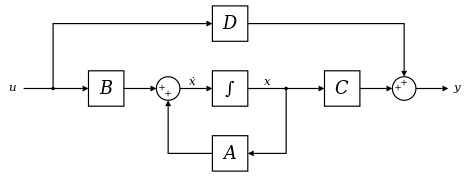
\includegraphics[scale=0.5]{C3.1_SSM.png}}
    \caption{Block diagram representation of Linear SSM}
    \label{ssm_bd}
\end{figure}

\subsection{Continuous-Time SSMs}
A continuous-time SSM is defined by the following system of differential equations:
\[
\begin{aligned}
\dot{\mathbf{x}}(t) &= \mathbf{A}(t)\mathbf{x}(t) + \mathbf{B}(t)\mathbf{u}(t) \\
\mathbf{y}(t) &= \mathbf{C}(t)\mathbf{x}(t) + \mathbf{D}(t)\mathbf{u}(t)
\end{aligned}
\]
where:
\begin{itemize}
    \item $\mathbf{x}(t) \in \mathbb{R}^n$ represents the system's state vector at time $t$, encapsulating its internal condition.
    \item $\mathbf{u}(t) \in \mathbb{R}^p$ represents the input vector or control variables at time $t$.
    \item $\mathbf{y}(t) \in \mathbb{R}^k$ represents the output vector containing the measurable quantities of interest at time $t$.
    \item $\dot{\mathbf{x}}(t) = \frac{d}{dt}\mathbf{x}(t)$ is the time derivative of the state vector.
    \item $\mathbf{A}(t) \in \mathbb{R}^{n \times n}$ is the state matrix, defining the system's internal dynamics.
    \item $\mathbf{B}(t) \in \mathbb{R}^{n \times p}$ is the input matrix, mapping the input to the state.
    \item $\mathbf{C}(t) \in \mathbb{R}^{k \times n}$ is the output matrix, mapping the state to the output.
    \item $\mathbf{D}(t) \in \mathbb{R}^{k \times p}$ is the feedthrough matrix, directly mapping the input to the output, like a skip connection.
\end{itemize}

\subsection{Linear Time-Invariant SSMs}
In the linear time-invariant (LTI) case, the matrices $\mathbf{A}$, $\mathbf{B}$, $\mathbf{C}$, and $\mathbf{D}$ remain constant over time, leading to a simpler representation:
\[
\begin{aligned}
\dot{\mathbf{x}}(t) &= \mathbf{A}\mathbf{x}(t) + \mathbf{B}\mathbf{u}(t) \\
\mathbf{y}(t) &= \mathbf{C}\mathbf{x}(t) + \mathbf{D}\mathbf{u}(t)
\end{aligned}
\]
These LTI systems have a crucial connection to convolutions, which is key to their efficient computation. We'll explore this relationship in more detail in the next section, while discussing S4.

\subsection{Discrete-Time SSMs}
Discrete-time SSMs model the evolution of a system at discrete time steps, representing the state and input as sequences. We are particularly interested in this, because they operate on discrete sequences of data, such as audio samples, image pixels, or text tokens.

\medskip

A discrete-time invariant SSM is defined as follows:
\[
\begin{aligned}
\mathbf{x}(t+1) &= \mathbf{A}\mathbf{x}(t) + \mathbf{B}\mathbf{u}(t) \\
\mathbf{y}(t) &= \mathbf{C}\mathbf{x}(t) + \mathbf{D}\mathbf{u}(t)
\end{aligned}
\]
where $t \in \mathbb{N}$ represents the discrete time steps, and the other terms are identical to the continuous-time SSM.

\medskip

To connect the continuous-time SSM to its discrete-time counterpart, we need to use a discretization procedure. Discretization involves transforming the continuous-time system parameters ($\mathbf{A}$, $\mathbf{B}$, $\mathbf{C}$, $\mathbf{D}$) into their discrete-time equivalents. This transformation is usually achieved using numerical integration methods. We discuss three commonly used discretization techniques in the upcoming sections.

\subsection{Euler Method}
The Euler method is a first-order numerical integration technique that approximates the derivative of a function using a forward difference. For the continuous-time SSM, the Euler method yields the following discrete-time update (for $\Delta \simeq 0$):
\[
\begin{aligned}
\mathbf{x}(t+\Delta) &\simeq \mathbf{x}(t) + \Delta \dot{\mathbf{x}}(t) \\
&= \mathbf{x}(t) + \Delta (\mathbf{A}\mathbf{x}(t) + \mathbf{B}\mathbf{u}(t)) \\
&= (\mathbf{I} + \Delta \mathbf{A})\mathbf{x}(t) + \Delta  \mathbf{B}\mathbf{u}(t)
\end{aligned}
\]
where $\Delta$ is the time step and $\mathbf{I}$ is the identity matrix. The output equation remains unchanged. Thus, the Euler method produces the discretized matrices as:
\[
\begin{aligned}
\mathbf{\overline{A}} &= (\mathbf{I} + \Delta\mathbf{A}) \\
\mathbf{\overline{B}} &= \Delta \mathbf{B}.
\end{aligned}
\]

\subsection{Bilinear Transform}
The bilinear transform offers improved accuracy over the Euler method. Applying the bilinear transform to the continuous-time SSM results in the following discrete-time update (for $\Delta \simeq 0$):
\[
\begin{aligned}
\mathbf{x}(t+ \Delta) &\simeq \left(\mathbf{I} - \frac{\Delta}{2}\mathbf{A}\right)^{-1} \left(\mathbf{I} + \frac{\Delta}{2}\mathbf{A}\right)\mathbf{x}(t) + \left(\mathbf{I} - \frac{\Delta}{2}\mathbf{A}\right)^{-1} \Delta \mathbf{B}\mathbf{u}(t).
\end{aligned}
\]

This gives the discretized matrices as:
\[
\begin{aligned}
\mathbf{\overline{A}} &= \left(\mathbf{I} - \frac{\Delta}{2}\mathbf{A}\right)^{-1} \left(\mathbf{I} + \frac{\Delta}{2}\mathbf{A}\right) \\
\mathbf{\overline{B}} &= \left(\mathbf{I} - \frac{\Delta}{2}\mathbf{A}\right)^{-1} \Delta \mathbf{B}.
\end{aligned}
\]


\subsection{Zero-Order Hold (ZoH)}
The ZoH method approximates the input signal as constant between time steps. This approach is simpler to implement and can be more efficient, but it might introduce some approximation errors. For the continuous-time SSM, the ZoH method yields the following discrete-time update (for $\Delta \simeq 0$):
\[
\begin{aligned}
\mathbf{x}(t+ \Delta) &\simeq e^{\Delta \mathbf{A}} \mathbf{x}(t) + (\Delta \mathbf{A})^{-1}(e^{\Delta \mathbf{A}} - \mathbf{I})(\Delta \mathbf{B}) \mathbf{u}(t)
\end{aligned}
\]
This gives the discretized matrices as:
\[
\begin{aligned}
\mathbf{\overline{A}} &= e^{\Delta \mathbf{A}} \\
\mathbf{\overline{B}} &= (\Delta \mathbf{A})^{-1}(e^{\Delta \mathbf{A}} - \mathbf{I})(\Delta \mathbf{B}).
\end{aligned}
\]

In the next section, we will focus on the S4 model, which is an SSM variant that utilizes the bilinear transform for discretization.


\section{S4}

The S4 model, introduced by Gu et al. \cite{s4}, stands out as a significant advancement in the field of SSMs. It addresses the computational limitations of previous SSM models, leading to a more efficient and effective approach to long-range dependency modelling.

\medskip

As discussed in \textbf{Section 3.2}, LTI SSMs are particularly interesting because they have a close connection to convolutions, which allows for efficient parallel training. The \textbf{S4 is a type of LTI SSM}. This means that its state matrix $\mathbf{A}$, input matrix $\mathbf{B}$, and output matrix $\mathbf{C}$ are all constant across time steps.

\medskip

To translate the continuous-time S4 model into a discrete-time form suitable for computation, the \textbf{Bilinear Transform} (discussed in \textbf{Section 3.1.5}) is employed. This choice is particularly beneficial for S4, as it allows for a more stable and efficient representation of the model.

\subsection{Training S4: Convolutional Representation}
LTI models (hence S4) can be expressed in terms of a convolution operation. This is a key advantage as it allows for parallelized training and efficient computations. Let's derive the convolutional representation for the LTI models.

Starting with the discrete-time SSM:\footnote{Here we are ignoring $\mathbf{D}$ because it is just a skip connection and does not affect the complexity of the calculation meaningfully.}
\[
\begin{aligned}
\mathbf{x}(t+1) &= \mathbf{A}\mathbf{x}(t) + \mathbf{B}\mathbf{u}(t) \\
\mathbf{y}(t) &= \mathbf{C}\mathbf{x}(t)
\end{aligned}
\]

Assuming an initial state of $\mathbf{x}(-1) = 0$, we can unroll the recurrence to get:
\[
\begin{aligned}
\mathbf{x}(0) &= \mathbf{B}\mathbf{u}(0) \\
\mathbf{x}(1) &= \mathbf{A}\mathbf{B}\mathbf{u}(0) + \mathbf{B}\mathbf{u}(1) \\
\mathbf{x}(2) &= \mathbf{A}^2\mathbf{B}\mathbf{u}(0) + \mathbf{A}\mathbf{B}\mathbf{u}(1) + \mathbf{B}\mathbf{u}(2) \\
&\vdots
\end{aligned}
\]

and similarly, the output:
\[
\begin{aligned}
\mathbf{y}(0) &= \mathbf{C}\mathbf{B}\mathbf{u}(0) \\
\mathbf{y}(1) &= \mathbf{C}\mathbf{A}\mathbf{B}\mathbf{u}(0) + \mathbf{C}\mathbf{B}\mathbf{u}(1) \\
\mathbf{y}(2) &= \mathbf{C}\mathbf{A}^2\mathbf{B}\mathbf{u}(0) + \mathbf{C}\mathbf{A}\mathbf{B}\mathbf{u}(1) + \mathbf{C}\mathbf{B}\mathbf{u}(2) \\
&\vdots
\end{aligned}
\]

This can be expressed as a convolution with kernel $\mathbf{K}$:
\[
\begin{aligned}
\mathbf{y} = \mathbf{u} * \mathbf{K}
\end{aligned}
\]

where
\[
\begin{aligned}
\mathbf{K} = (\mathbf{C}\mathbf{B}, \mathbf{C}\mathbf{A}\mathbf{B}, \mathbf{C}\mathbf{A}^2\mathbf{B}, \dots)
\end{aligned}
\]

This convolutional form is crucial because it allows for efficient parallelized computation by pre-computing the kernel $\mathbf{K}$, and allows us to avoid the recurrence of LTIs.

\subsection{Challenges with Naive Implementation}
The naive implementation of the convolution kernel involves repeatedly multiplying the matrix $\mathbf{A}$ by the vector $\mathbf{B}$. This requires $\mathcal{O}(N^2L)$ operations and $\mathcal{O}(NL)$ space for a state dimension $N$ and sequence length $L$. This complexity quickly becomes prohibitive as the sequence length grows, especially for larger SSMs (where $N$ might be 100 or more).

\subsection{Adding Further Structure to A}
To address the computational challenges of computing $\mathbf{K}$, Gu et al. \cite{s4} propose adding structure to the state matrix $\mathbf{A}$. This structure makes it possible to efficiently compute both the convolutional representation ($\mathbf{K}$) and the recurrent update rule for the state vector. The key idea behind S4 is to use a \textbf{Normal Plus Low-Rank} (NPLR) representation for $\mathbf{A}$, which we discuss next.

\subsubsection{Using HIPPO Matrix}
Gu et al. \cite{hippo,s4} proposed a specific structure for $\mathbf{A}$, known as the \textbf{HIPPO matrix}, which has a remarkable connection to orthogonal polynomial projections and time-invariant SSMs. The HIPPO matrix is defined as:
\[
\begin{aligned}
\mathbf{A}_{nk} =
-\begin{cases}
(2n + 1)^{\frac{1}{2}}(2k + 1)^{\frac{1}{2}} & \text{if } n > k \\
n + 1 & \text{if } n = k \\
0 & \text{if } n < k
\end{cases}
\end{aligned}
\]

This matrix has the NPLR property that allows for efficient computation of the SSM kernel, even for long sequences. Its NPLR form is as follows:
\[
\begin{aligned}
\mathbf{A} = \mathbf{V}\mathbf{\Lambda}\mathbf{V}^* - \mathbf{P}\mathbf{Q}^T,
\end{aligned}
\]
where:
\begin{itemize}
    \item $\mathbf{V} \in \mathbb{C}^{\mathbf{N} \times \mathbf{N}}$ is a unitary matrix,
    \item $\mathbf{\Lambda}$ is a diagonal matrix,
    \item $\mathbf{P}, \mathbf{Q} \in \mathbb{R}^{\mathbf{N} \times r}$, with $r=1$ for HIPPO.
\end{itemize}

\subsubsection{Complexity Improvements}
As shown by the authors in the S4 paper \footnote{Refer to \textbf{Theorem 2} and \textbf{Theorem 3} of \textbf{Section 3.3} of the S4 Paper \cite{s4}}, this NPLR parameterisation of the $\mathbf{A}$ matrix leads to significant improvements in computational complexity, both in recurrent and convolutional modes:
\begin{itemize}
    \item \textbf{Recurrent Mode Complexity}: Computing one step of the recurrence with a NPLR matrix $\mathbf{A}$ requires only $\mathbf{\mathcal{O}(N)}$ operations, making it computationally efficient.
    \item \textbf{Convolution Mode Complexity}: The S4 kernel computation involves evaluating the generating function of $\mathbf{K}$ at specific points, which can be done efficiently in $\mathbf{\tilde{\mathcal{O}}(N+L)}$ operations (where $L$ is the sequence length) using a black-box Cauchy kernel computation. This complexity makes it optimal for efficient kernel pre-computation and helps in avoiding the recurrence of S4.
\end{itemize}

\begin{table}[h!]
\centering
\begin{tabular}{lcccc}
\toprule
 & \textbf{Convolution} & \textbf{Recurrence} & \textbf{Attention} & \textbf{S4} \\
\midrule
\textbf{Parameters} & $LH$ & $H^2$ & $H^2$ & $H^2$ \\
\textbf{Training} & $\tilde{L}H(B + H)$ & $BLH^2$ & $B(L^2 H + LH^2)$ & $BH(\tilde{H} + \tilde{L}) + B\tilde{L}H$ \\
\textbf{Space} & $BLH$ & $BLH$ & $B(L^2 + HL)$ & $BLH$ \\
\textbf{Parallel} & Yes & No & Yes & Yes \\
\textbf{Inference} & $LH^2$ & $H^2$ & $L^2 H + H^2 L$ & $H^2$ \\
\bottomrule
\end{tabular}
\caption{Complexity of various sequence models in terms of sequence length ($L$), batch size ($B$), and hidden dimension ($H$); tildes denote log factors. Metrics are computation for 1 sample and time-step. For simplicity, the state size of S4 $N = H$. Convolutions are efficient for training while recurrence is efficient for inference, while SSMs combine the strengths of both.}
\label{tab:complexity}
\end{table}

\subsection{Architecture of Deep S4}
The S4 model can be incorporated into deep neural network architectures, similar to other sequence models, to improve its expressivity and ability to learn complex features. Here are some key aspects of the deep S4 architecture:
\begin{itemize}
    \item \textbf{Multi-Channel Support}: For inputs with multiple features (channels/dimensions), S4 uses separate, independently trained models for each channel.
    \item \textbf{Parameter Tying}: The state matrix $\mathbf{A}$, input matrix $\mathbf{B}$, and timescale parameter $\Delta$ can be tied across different channels to reduce the number of parameters.
    \item \textbf{Linear Mixing}: After each S4 layer, a linear feed-forward layer is applied to mix the outputs from different channels.
    \item \textbf{Nonlinear Activations}: A non-linear activation function, such as GELU, is commonly used between S4 layers.
    \item \textbf{Residual Connections}: Residual connections are employed to improve information flow and mitigate vanishing gradients in deep networks.
    \item \textbf{Normalization}: Layer Normalization or Batch Normalization is often used to stabilize training and enhance generalization.
\end{itemize}

\subsection{Empirical Performance in LRA}
The S4 model has achieved significant performance improvements on the LRA benchmark \cite{lra}, particularly for tasks requiring long-range dependencies. It has demonstrated the \textbf{first successful solution} for the challenging Path-X task\footnote{more details in \textbf{Section 1.2.1}} in the LRA benchmark as shown in \ref{s4-lra}. This showcases the S4 model's effectiveness in addressing long-range dependency challenges.

\begin{figure}[ht]
    \centerline{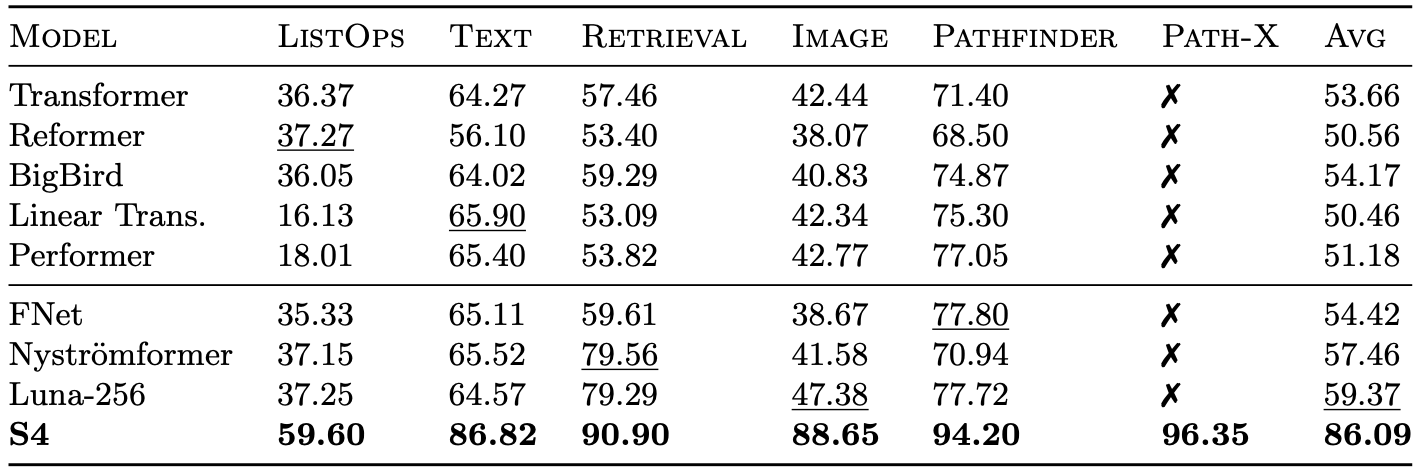
\includegraphics[scale=0.6]{C3.2.5_S4_LRA.png}}
    \caption{Original Transformer (Top) variants vs S4 (Bottom) in LRA}
    \label{s4-lra}
\end{figure}

\subsection{Limitations of S4 and LTIs in Language Modelling}
While S4 excels in various domains, it has limitations in language modelling. This is primarily due to its inability to perform content-based reasoning, which is crucial for language modelling tasks. Here are two key examples illustrating this limitation:
\begin{itemize}
    \item \textbf{Selective Copying}: S4 struggles with tasks like Selective Copying, where it needs to selectively remember and copy relevant tokens while filtering out irrelevant ones.
    \item \textbf{Induction Heads}: S4 also faces difficulties with Induction Heads tasks, which require the model to recall specific tokens based on contextual cues.
\end{itemize}

To address these limitations in LTIs, more recent SSM Models like Mamba \cite{mamba} were developed.

\begin{figure}[ht]
    \centerline{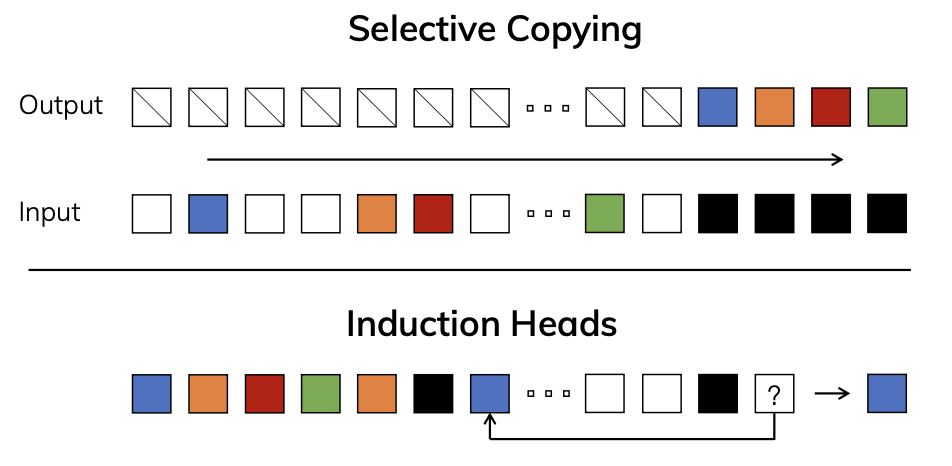
\includegraphics[scale=0.75]{C3.2.6_SelectiveC_InductionH.png}}
    \caption{ The standard version of the Copying task involves constant spacing between input and output elements and is easily solved by LTIs. (Top) The Selective Copying task has random spacing in between inputs and requires time-varying models that can selectively remember or ignore inputs depending on their content. (Bottom) The Induction Heads task is an example of associative recall that requires retrieving an answer based on context, a key ability for LLMs.}
    \label{selective-copy-induction-heads}
\end{figure}

\chapter{Selective SSM and Mamba}

While S4 \cite{s4} provides a powerful framework for capturing LRDs in sequence modelling, it has limitations in certain data modalities, especially those involving discrete and information-dense sequences like text. This is primarily due to S4's reliance on time-invariant (LTI) dynamics, where the model parameters are fixed across all time steps. This constraint hinders S4's ability to reason about the specific content of the sequence and make input-dependent decisions.

\medskip

This chapter introduces Selective State Space Models (S6) \cite{mamba}, a class of SSMs that address this limitation by incorporating a selection mechanism. This mechanism allows the model to dynamically adjust its parameters based on the current input token, enabling it to selectively propagate or forget information along the sequence length dimension. We begin by discussing how to modify S4 to introduce this selection mechanism, emphasizing the key differences in its computation and parameterization. We then present Mamba \cite{mamba}, a simplified SSM architecture incorporating selective state spaces and a specialized block design that eliminates the need for attention or even MLP layers.

\section{S6}

The S6 model \cite{mamba} is a modified version of S4 \cite{s4} that incorporates a selection mechanism to address the limitations of LTI SSMs, especially in handling discrete modalities like text. This section delves into the key aspects of S6.

\subsection{Discretization Strategy: ZoH}
While S4 utilizes the bilinear transform for discretization, S6 adopts the Zero-Order Hold (ZoH) method. This shift offers a more convenient implementation for introducing selectivity and enables better understanding of the selection mechanism.

Recall from \textbf{Section 3.1.6} that the ZoH method assumes a constant input signal between discrete time steps. This results in the following discretized update equation for S6:
\[
\begin{aligned}
\mathbf{x}(t+ \Delta) &\simeq e^{\Delta \mathbf{A}} \mathbf{x}(t) + (\Delta \mathbf{A})^{-1}(e^{\Delta \mathbf{A}} - \mathbf{I})(\Delta \mathbf{B}) \mathbf{u}(t)
\end{aligned}
\]
where:
\begin{itemize}
    \item $\mathbf{\overline{A}} = e^{\Delta \mathbf{A}}$ is the discretized state matrix,
    \item $\mathbf{\overline{B}} = (\Delta \mathbf{A})^{-1}(e^{\Delta \mathbf{A}} - \mathbf{I})(\Delta \mathbf{B})$ is the discretized input matrix,
    \item $\Delta$ is the time step.
\end{itemize}

\subsection{Breaking LTI: Adding Selectivity}
The key to S6 lies in making the model's parameters time-dependent and input-aware. This is achieved by making the timescale parameter $\Delta$ and the input and output projection matrices $\mathbf{B}$ and $\mathbf{C}$ functions of the current input token.

\medskip

Specifically, let $\mathbf{u}$ denote the input. The S6 update equation with selectivity is given as:
\[
\begin{aligned}
\mathbf{x}(t+1) &= \mathbf{\overline{A}}(t) \mathbf{x}(t) + \mathbf{\overline{B}}(t) \mathbf{u}(t) \\
\mathbf{y}(t) &= \mathbf{C}(t) \mathbf{x}(t) + \mathbf{D}(t) \mathbf{u}(t)
\end{aligned}
\]
where:
\begin{itemize}
    \item $\Delta(t)$ is the timescale parameter, also a function of the current input token (with shape $(B, L, D)$).
    \item $\mathbf{\overline{A}}(t)$ is the discretized state matrix \footnote{$\mathbf{A}$ matrix is still constant with fixed initialization} (now time-dependent because of it's dependence on $\Delta(t)$).
    \item $\mathbf{\overline{B}}(t)$ is the discretized input matrix (now time-dependent because of it's dependence on time dependent $\mathbf{B}(t)$ and $\Delta(t)$).
    \item $\mathbf{C}(t)$ and $\mathbf{D}(t)$ are also time-dependent by initialization.
\end{itemize}

Specifically, in the S6 layer, $\mathbf{B}(t)$, $\mathbf{C}(t)$, $\mathbf{D}(t)$ and $\Delta(t)$ are linear projections of the current input token $\mathbf{u}(t)$ as follows:
\begin{itemize}
    \item $\mathbf{B}(t) = Linear_N(\mathbf{u}(t))$,
    \item $\mathbf{C}(t) = Linear_N(\mathbf{u}(t))$,
    \item $\mathbf{D}(t) = Linear_N(\mathbf{u}(t))$
    \item $\Delta(t) = Broadcast_D(Linear_1(\mathbf{u}(t)))$.
\end{itemize}

Here, $Linear_d$ represents a parameterized (and learnable) linear projection to dimension $d$, and $Broadcast_D$ expands the output of a linear layer to dimension $D$ by replicating each element.

\subsection{Adding Structure to A}
Even though the state matrix $\mathbf{A}$ remains constant, the time-dependent nature of the discretization step introduces input-dependence to the discretized $\mathbf{A}$ matrix. This requires us to impose structure on $\mathbf{A}$ to ensure efficient computation. A recent work by Gu et al. \cite{dssm} showed that diagonal state spaces are as effective as the structured state spaces used in S4 \cite{s4}.

\begin{figure}[ht]
    \centerline{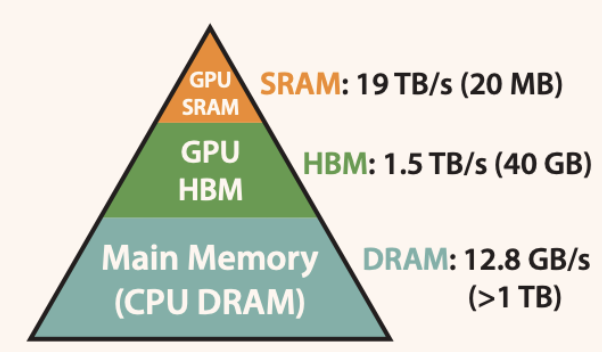
\includegraphics[scale=0.6]{C4.1.3_GPU_Band.png}}
    \caption{Memory Heirarchy with Bandwidth and Size}
    \label{gpu-band}
\end{figure}

\begin{itemize}
    \item \textbf{S4D-Lin-Complex and S4D-Real Initializations}: For S6, we typically use the S4D-Lin-Complex or S4D-Real initializations for the state matrix $\mathbf{A}$, derived from the HIPPO framework \cite{hippo}. These initializations are well-suited for capturing long-range dependencies and offer a balance between expressivity and computational efficiency.
    \begin{itemize}
        \item \textbf{S4D-Lin-Complex}: This initialization sets the diagonal elements of $\mathbf{A}$ as $A_k = -1/2 + i k$.
        \item \textbf{S4D-Real}: This initialization sets the diagonal elements of $\mathbf{A}$ as $A_k = -(k+1)$. It is a real-valued initialization that avoids complex arithmetic and can achieve comparable performance. The selection of complex or real initializations depends on the specific task and its computational constraints.
    \end{itemize}
    \item \textbf{Improving Recurrence with Associative Parallel Scan and Hardware Optimizations}: The selective nature of S6 prevents the use of efficient convolution-based computations enabled by LTIs. Therefore, the recurrent computation using a parallel scan \cite{mamba} is adopted. However, directly applying the scan operation to the full state matrix can be inefficient due to its large size of scan input $(\overline{\mathbf{A}}, \overline{\mathbf{B}})$ of size $(B, L, D, N)$. To mitigate this, a hardware-aware algorithm is used that leverages the GPU's memory hierarchy. 
    
    Concretely, instead of preparing the scan input in GPU High-Bandwidth Memory (HBM), we directly load the SSM parameters, i.e. $\mathbf{A}, \mathbf{B}, \mathbf{C}, \mathbf{D}$ and $\Delta$ directly from slow HBM to fast SRAM, to perform the discretization and recurrence directly in SRAM and write the results back to HBM. This minimizes memory transfers between HBM and SRAM, thereby enhancing speed \footnote{This is similar to what happens in the FlashAttention \cite{flashattn} implementation of Transformers}. This is achieved via:
    \begin{itemize}
        \item \textbf{Kernel Fusion}: The discretization, scan, and output projection operations are fused into a single kernel, reducing memory I/O operations and improving speed.
        \item \textbf{Recomputation}: Instead of storing the intermediate states, which consume significant memory, they are recomputed during the backward pass. This minimizes memory overhead and accelerates training.
    \end{itemize}
\end{itemize}

\section{Mamba}

The Mamba model \cite{mamba} builds upon the S6 architecture (which incorporates selection and scan mechanisms into S4) and takes a step further by simplifying the overall architecture and introducing a novel, hardware-aware implementation. This section delves into the core aspects of Mamba.

\subsection{Architecture}

Mamba simplifies the architecture of traditional SSM models, eliminating the need for attention or even vanilla MLP blocks. It achieves this by combining the SSM block with a gated MLP block into a single, homogeneous block design. This design effectively integrates the strengths of both SSMs and MLPs, resulting in a more efficient and streamlined architecture.

\begin{figure}[ht]
    \centerline{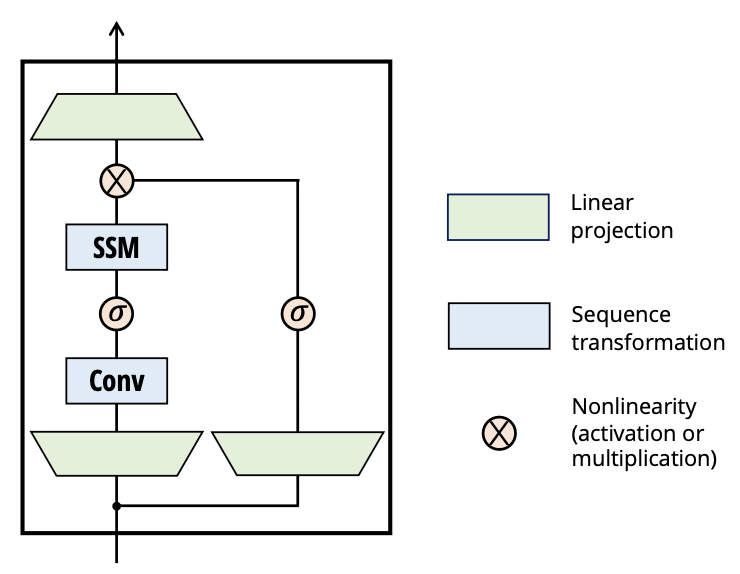
\includegraphics[scale=0.6]{C4.2.1_Mamba_Arch.png}}
    \caption{This represents a single Mamba Block, which can be stacked to form a deep Mamba model.}
    \label{mamba-arch}
\end{figure}

The Mamba Block, as shown in \ref{mamba-arch} consists of two branches:
\begin{itemize}
    \item \textbf{SSM Branch}: The main branch processes the input sequence using a selective SSM layer (S6).
    \item \textbf{MLP Branch}: A gated MLPs block is applied in parallel to the SSM branch. This block uses a gated mechanism (SwiGLU) to enhance its expressivity and performance in long sequence modeling.
\end{itemize}

The outputs of both branches are then combined through element-wise multiplication, followed by a final linear projection. This design allows for efficient processing of long sequences while leveraging the computational advantages of both SSMs and MLPs.

\subsection{Empirical Results}

Mamba has achieved impressive results across diverse tasks and modalities, showcasing its potential as a general sequence modeling backbone. We highlight two key areas:

\subsubsection{Scaling Laws}

\begin{figure}[ht]
    \centerline{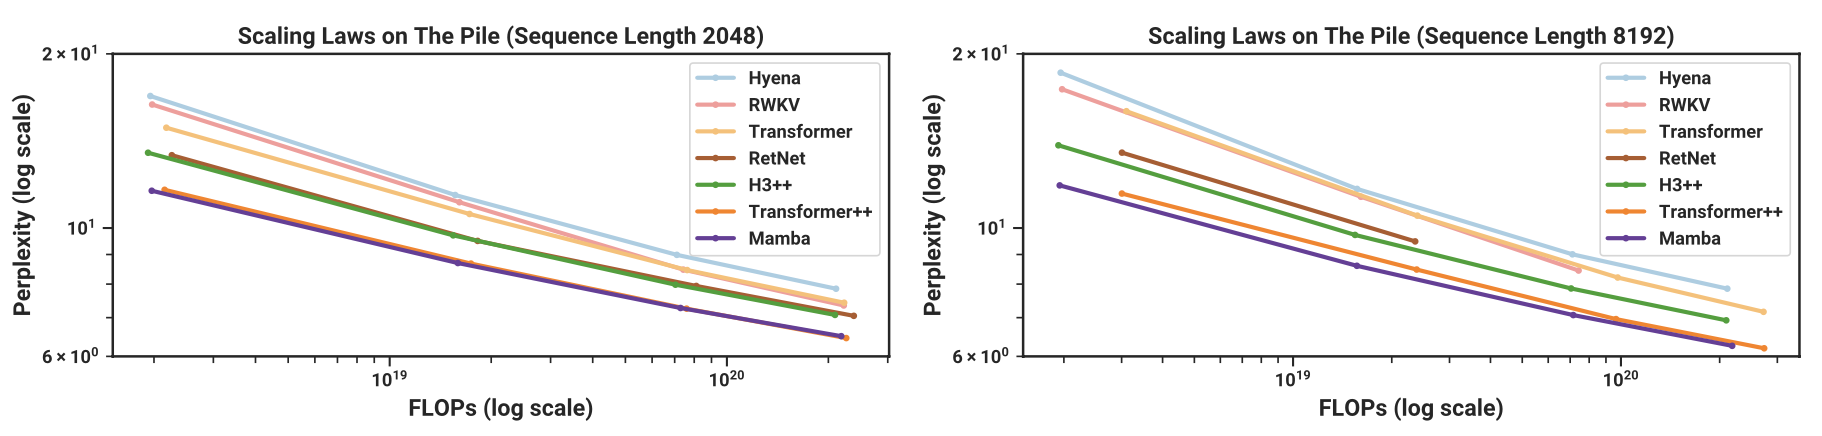
\includegraphics[scale=0.5]{C4.2.2_Mamba_Scaling.png}}
    \caption{Scaling Laws of models with sizes from $125M - 1.3B$ parameters, trained on Pile Dataset \cite{pileds}.}
    \label{mamba-scale}
\end{figure}

As evident from \ref{mamba-scale}, Mamba seems to scale better than all other attention-free models (like Hyena and RWKV) and is the first to match the performance of a very strong Transformer recipe\footnote{This like LLaMA \cite{llama} using RoPE, SwiGLU MLP, RMSNorm (instead of LayerNorm), no linear bias, and higher Learning Rate} (which they call Transformer++).

\subsubsection{Efficiency Benchmarks}

\begin{figure}[ht]
    \centerline{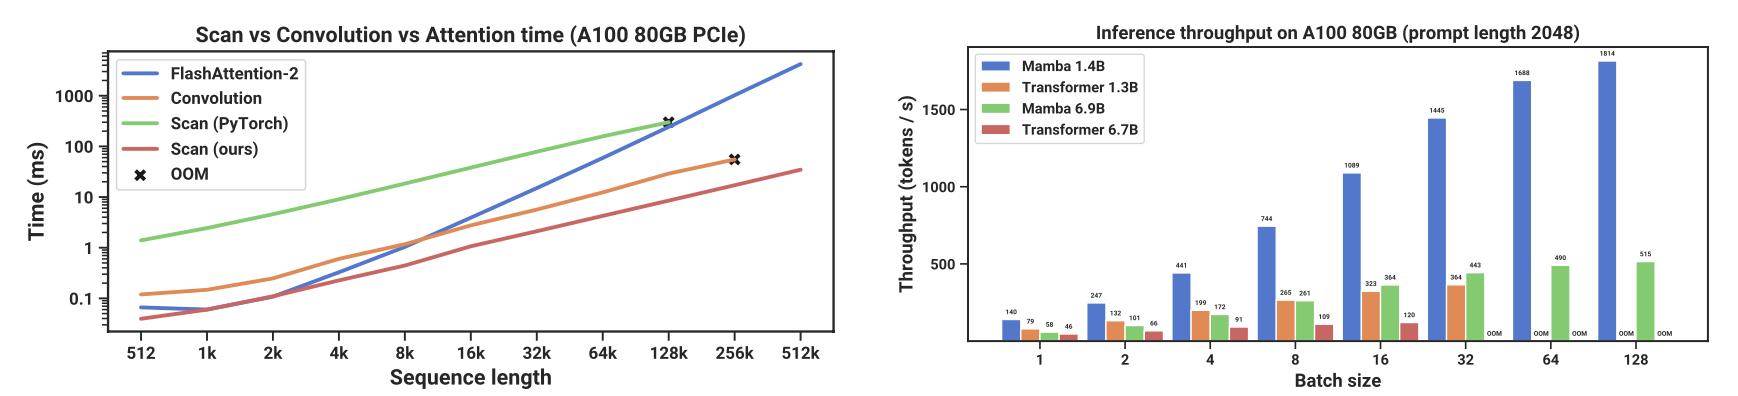
\includegraphics[scale=0.55]{C4.2.2_Mamba_Eff.png}}
    \caption{(Left) Training Times (Right) Inference Times of Mamba vs Transformers}
    \label{mamba-eff}
\end{figure}

From \ref{mamba-eff}, we can see that Mamba is significantly faster than Transformers, especially during inference. The hardware-aware algorithm for the parallel scan\footnote{The S6 Recurrence in Mamba} operation makes it faster than the standard scan implementation in PyTorch, promising a speedup of almost 20-40x. In terms of inference throughput, Mamba achieves remarkably higher throughput than Transformers of the same size, promising 4-5x higher inference throughput with similar memory footprint.

\bigskip

These empirical results strongly suggest that Mamba offers a compelling alternative to Transformers, particularly in domains demanding efficient long-sequence modeling.


\chapter{Linear Recurrent Units: Simplicity and Universality}

The impressive performance of SSMs on LRD tasks sparked a natural question: "\textbf{Could this level of performance be achieved with a simpler model?}" Researchers turned their attention to RNNs with linear recurrences, investigating if careful design and parameterization, guided by principles learnt from S4's success, could reach comparable results without the complex mathematical machineries of SSMs.

\medskip

This chapter delves into this exploration, starting with a discussion on the theoretical universality of RNNs when combined with non-linear projections. We then introduce Linear Recurrent Units (LRUs) \cite{lru}, showcasing how a systematic series of modifications to vanilla RNNs can lead to comparable performance to S4 on the LRA benchmark \cite{lra}.

\section{Universality of Linear RNN followed by Non-Linear Projections}

\begin{figure}[ht]
    \centerline{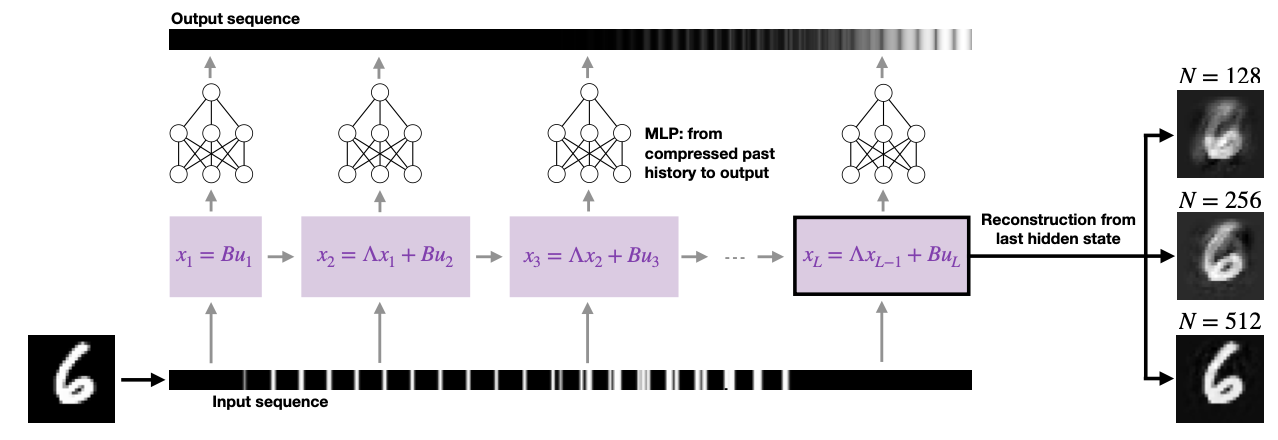
\includegraphics[scale=0.6]{C5.1_Universality_LRNN.png}}
    \caption{Example: Linear RNN + position-wise MLP for flattened MNIST digits reconstruction. The role of linear RNN is to compress and store the input sequence into the hidden states, from which we can recover past tokens using a MLP. As hidden size $N$ increases, the reconstruction becomes more and more faithful.}
    \label{univ-rnn}
\end{figure}

Orvieto et al. \cite{universality_lrnn} proved that even basic architectures, combining linear RNNs and position-wise MLPs, are theoretically universal function approximators for sequences. Their key insight is that these two components have distinct roles: the linear RNN acts as a compressor, encoding the entire input history into a fixed-size hidden state, while the MLP acts as a non-linear processor, extracting complex patterns from this compressed representation.

\medskip

This universality hinges on two conditions:
\begin{itemize}
    \item \textbf{Proper Initialization}: The RNN's state matrix must be initialized such that its eigenvalues lie close to the unit circle in the complex plane. This ensures the RNN can effectively capture long-range dependencies.
    \item \textbf{Sufficient Width}: Both the RNN and MLP need to be wide enough to accommodate the complexity of the target function.
\end{itemize}

This result highlights:
\begin{itemize}
    \item \textbf{Simplicity and Efficiency}: Linear recurrences, combined with MLPs, are sufficient for universality, which can lead to computationally efficient models due to the parallelizability of linear RNNs\footnote{parallelizability of Linear RNNs stem from the fact that they belong to the family of LTI SSMs}.
    \item \textbf{Power of Complex Numbers}: Using complex values in the recurrence can improve the stability and effectiveness of the RNN's compression by allowing more control over the eigen-values.
\end{itemize}

\section{LRU}

The Linear Recurrent Unit (LRU), introduced by Orvieto et al. \cite{lru}, is a carefully designed RNN architecture that leverages the theoretical universality of linear recurrences combined with non-linear projections to achieve strong performance. The LRU achieves this by systematically incorporating a series of modifications to a vanilla RNN, each designed to enhance its stability, efficiency, and ability to capture LRDs.

\medskip

In the next few sections, we discuss the strategies employed to design a performant deep RNN architecture, which can achieve performance comparable to SSMs on LRA tasks.

\subsection{Linear Recurrences}

\begin{figure}[ht]
    \centerline{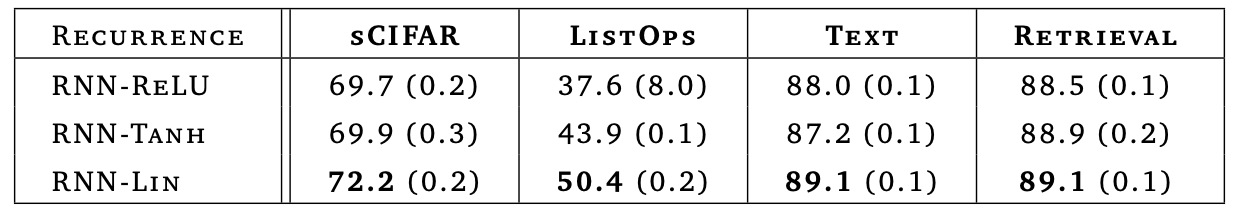
\includegraphics[scale=0.6]{C5.2.1_LRNN_Perf.png}}
    \caption{Effect of removing the non-linearity from the recurrence on the feasible LRA tasks.}
    \label{lrnn-perf}
\end{figure}

The first key step is to linearize the recurrence, a seemingly counterintuitive move given the widespread belief that non-linearities within the recurrence are crucial for RNNs to model complex functions. However, as evident from \ref{lrnn-perf}, in the context of deep architectures interleaved with non-linear MLPs, dropping the non-linearity in the recurrence actually boosted performance on LRA tasks \cite{lra}. This seemingly paradoxical finding aligns with the theoretical universality result \cite{universality_lrnn} and the observation that non-linear projections applied after the linear RNN can be expressive, enabling the model to capture complex non-linear dynamics.

\medskip

By switching to linear recurrences, LRUs gain several advantages:
\begin{itemize}
    \item \textbf{Explicit Gradient Control}: The removal of non-linearities allows for direct control over how quickly gradients might vanish or explode. This is crucial for learning LRDs, as it enables careful tuning of the eigenvalues in the recurrent matrix to mitigate vanishing gradients.
    \item \textbf{Parallelizable Training}: Linear recurrences can be efficiently parallelized during training, leading to substantial speedups over non-linear RNNs which require sequential computation.
\end{itemize}

\subsection{Complex Diagonal Recurrent Matrices}
Building on the insights from S4 \cite{s4}, LRUs also adopt the use of complex-valued diagonal recurrent matrices. This choice, while seemingly unusual for traditional RNNs, brings significant computational advantages and aligns with the theoretical findings on the benefits of complex numbers in linear recurrences \cite{universality_lrnn}.


\subsubsection{Switching to Diagonal Matrices}

Diagonal matrices offer substantial computational advantages due to their simplified structure. Let's examine how we can transform a dense linear RNN into its diagonal form without affecting expressivity.

\medskip

We start with the recurrence of a linear RNN:
\[
\begin{aligned}
\mathbf{x}_k &= \mathbf{A}\mathbf{x}_{k-1} + \mathbf{B}\mathbf{u}_k,
\end{aligned}
\]
where $\mathbf{A} \in \mathbb{R}^{N \times N}$ is the recurrent matrix, $\mathbf{B} \in \mathbb{R}^{N \times D}$ is the input projection matrix, $\mathbf{x} \in \mathbb{R}^N$ is the hidden state, and $\mathbf{u} \in \mathbb{R}^{D}$ is the input. Assuming $\mathbf{x}_{-1} = 0$, we can unroll the recurrence as:
\[
\begin{aligned}
\mathbf{x}_k = \sum^{k-1}_{j=0}\mathbf{A}^j \mathbf{B} \mathbf{u}_{k-j}.
\end{aligned}
\]

The exponentiation of $\mathbf{A}$ in this equation is the source of the vanishing/exploding gradient issue in RNNs. To better understand this, we leverage an eigenvalue analysis. Almost every matrix $\mathbf{A} \in \mathbb{R}^{N \times N}$ is diagonalizable\footnote{The set of non-diagonalizable matrices has measure zero}, meaning we can write it as $\mathbf{A} = \mathbf{P}\mathbf{\Lambda}\mathbf{P}^{-1}$, where $\mathbf{P} \in \mathbb{C}^{N \times N}$ is an invertible matrix, and $\mathbf{\Lambda} = \text{diag}(\lambda_1, \lambda_2, ..., \lambda_N) \in \mathbb{C}^{N \times N}$ is a diagonal matrix containing the eigenvalues of $\mathbf{A}$. Note that, unlike symmetric matrices where eigenvalues and eigenvectors are real, non-symmetric matrices may have complex eigenvalues and eigenvectors.

\medskip

Plugging this decomposition into the unrolled recurrence and multiplying both sides by $\mathbf{P}^{-1}$, we obtain:
\[
\begin{aligned}
\mathbf{P}^{-1}\mathbf{x}_k = \sum^{k-1}_{j=0}\mathbf{\Lambda}^j \mathbf{P}^{-1} \mathbf{B} \mathbf{u}_{k-j}.
\end{aligned}
\]

By renaming $\overline{\mathbf{x}_k} \leftarrow \mathbf{P}^{-1}\mathbf{x}_k$ and $\overline{\mathbf{B}} \leftarrow \mathbf{P}^{-1}\mathbf{B}$, we arrive at a diagonal recurrence in the complex domain:
\[
\begin{aligned}
\overline{\mathbf{x}_k} = \sum^{k-1}_{j=0}\mathbf{\Lambda}^j\overline{\mathbf{B}} \mathbf{u}_{k-j}.
\end{aligned}
\]

Finally, the output of the RNN can be computed as:
\[
\begin{aligned}
\mathbf{y}_k = \text{Re}[\overline{\mathbf{C}}\mathbf{x}_k] + \mathbf{D}\mathbf{u}_k,
\end{aligned}
\]
where $\overline{\mathbf{C}} = \mathbf{C}\mathbf{P}^{-1}$, and we take the real part of $\mathbf{C}\mathbf{x}_k$. Therefore, we can learn $(\mathbf{\Lambda}, \overline{\mathbf{B}}, \overline{\mathbf{C}}, \mathbf{D})$ instead of $(\mathbf{A}, \mathbf{B}, \mathbf{C}, \mathbf{D})$, where $\mathbf{\Lambda},\overline{ \mathbf{B}}, \overline{\mathbf{C}}$ are complex-valued and $\mathbf{\Lambda}$ is diagonal.

\medskip

This diagonal form allows for significant speedups both during training and inference as exponentiating a diagonal matrix simply involves exponentiating its diagonal elements, a trivial operation. Furthermore, unlike non-linear recurrences which need sequential computation, linear recurrences can be parallelized using efficient associative scans (as in S4 \cite{s4} and Mamba \cite{mamba}).

\subsubsection{Controlling Stability with Eigenvalues}
Recall that the diagonalized recurrence is given by:
$\overline{\mathbf{x}_k} = \sum^{k-1}_{j=0}\mathbf{\Lambda}^j\overline{\mathbf{B}} \mathbf{u}_{k-j}$. Focusing on the $j$-th component of the hidden state at timestamp $k$, we observe its evolution as:

\[ |x_{k,j}| = \mathcal{O}(|\overline{x}_{k-1,j}|) = \mathcal{O}(|\lambda_j|^k). \]

This equation clearly shows that the magnitude of the $j$-th eigenvalue, $|\lambda_j|$, directly determines the rate at which the signal from past inputs decays or grows in the corresponding hidden state dimension.

\medskip

This leads us to the following observations:
\begin{itemize}
    \item If $|\lambda_j| < 1$, the signal decays exponentially with each time step, leading to vanishing gradients and a limited ability to capture LRDs.
    \item If $|\lambda_j| > 1$, the signal grows exponentially, potentially leading to exploding gradients and numerical instability during training.
\end{itemize}

\medskip

Therefore, to ensure stability and facilitate learning of LRDs, LRUs constrain the eigenvalues to lie within the unit circle, i.e., $|\lambda_j| < 1$ for all $j$. This constraint ensures that the influence of past inputs gradually decays, preventing exploding gradients while still allowing information from the distant past to contribute to the current state. This is exactly what the Glorot Equivalent Initialization achieves, as we see in the next section.


\subsubsection{Glorot Equivalent Initialization}
To ensure a fair comparison with vanilla RNNs, Orvieto et al. \cite{lru} sought an initialization for the diagonal system that preserved the eigenvalue spectrum of a \textbf{Glorot-initialized dense RNN}. A Glorot initialized matrix \cite{glorotinit} $\mathbf{A} \in \mathbb{R}^{N \times N}$ is such that each entry of $\mathbf{A}$ is sampled independently from a Gaussian with mean $0$ and variance $\frac{1}{N}$. By leveraging the \textbf{Strong Circular Law}\footnote{Refer to \textbf{Theorem 3.1} of LRU paper \cite{lru} for more details}, we know that the eigenvalues of a Glorot-initialized dense RNN are uniformly distributed within the unit circle in the complex plane.

\medskip

This leads to a simple yet effective initialization strategy for LRUs: sampling the diagonal elements of the recurrent matrix uniformly from the \textbf{unit disk in the complex plane}.

\subsubsection{Stable Exponential Parameterization}
To further enhance stability and control over gradient flow, LRUs introduced a stable exponential parameterization for the diagonal elements of the recurrent matrix. This involved representing each diagonal element as the exponential of a complex number, decoupling magnitude and phase:
\[\lambda_j = \exp(-\exp(v_j^{log}) + i \exp(\theta_j^{log})),\]
where:
\begin{itemize}
    \item $\exp(-\exp(v_j^{log}))$ is the magnitude, controlled by the learnable parameter $v_j^{log}$.
    \item $\exp(\theta_j^{log})$ is the phase, controlled by the learnable parameter $\theta_j^{log}$.
\end{itemize}

\paragraph{Optimization under Exponential Parameterization} 
This exponential parameterization offers several advantages:
\begin{itemize}
    \item \textbf{Decoupled Magnitude and Phase}: It decouples the learning of magnitude and phase, making optimization easier and more stable, especially when using optimizers like Adam.
    \item \textbf{Explicit Stability Control}: The exponential form ensures that the magnitude of each eigenvalue is always less than 1\footnote{$0 < e^{-|x|} \le 1$ for all $x \in \mathbb{R}$}, guaranteeing stability and mitigating exploding gradients. To further enforce stability and allow for exploration of \textbf{initializations closer to the unit circle}, LRUs employ an additional exponential non-linearity on the magnitude, hence the double exponential. By initializing the eigenvalues closer to the unit circle, LRUs can be biased towards capturing longer-range interactions, further improving their performance on LRD tasks.
    \item \textbf{Reducing Eigenvalue Phase at Initialization}: For very long sequences, initializing the eigenvalues with a uniform phase distribution\footnote{This means uniformly sampling from $[0,2\pi]$}, can lead to the model learning spurious high-frequency oscillations, hindering its ability to capture global patterns. To address this, LRUs restrict the phase of the eigenvalues at initialization to a small range around 0, encouraging the model to learn more global, low-frequency features relevant for long-range reasoning. This can be done by initializing the phase parameter as $\exp(\theta_j^{log})$, which can ensure small phases by initializing the learnable $\theta_j^{log}$ to be negative.
\end{itemize}

To address the challenges of learning very long-range dependencies, especially those encountered in the PathX task, LRUs incorporate another key modification:

\subsubsection{Normalization}
As the eigenvalues of the recurrent matrix approach the unit circle, the \textbf{norm of the hidden state can potentially explode} during the forward pass\footnote{For more details check \textbf{Proposition 3.3 Forward-pass blow-up} in the LRU paper \cite{lru}. This says that as we approach the unit circle in the limit, $\mathbb{E}|x_k|^2 \xrightarrow{\infty} \sum_{i=0}^{\infty} |\lambda|^{2i} = \frac{1}{1-|\lambda|^2}$}. To counteract this, LRUs introduced a normalization factor $\gamma \in \mathbb{R}^{N}$ for each dimension, initialized element-wise as $\gamma_{i} \leftarrow \sqrt{1 - |\lambda_i|^2}$, which modifies the recurrence as:
\[\mathbf{x}_k = \mathbf{\Lambda} \mathbf{x}_{k-1} + \mathbf{\gamma} \odot \mathbf{B} \mathbf{u}_k, \]
where $\odot$ represents element-wise multiplication.

\subsection{Deep LRU Architecture}
The deep LRU architecture mirrors the general structure of deep SSMs and Transformers, incorporating residual connections, layer normalization, and non-linear mixing layers. The core difference lies in replacing the SSM or attention block with an LRU layer, parameterized as follows:
\[\mathbf{x}_{k} = \mathbf{diag(\lambda)}\mathbf{x}_{k-1} + \mathbf{\gamma} \odot \mathbf{B}\mathbf{u}_{k},\]
where:
\begin{itemize}
    \item $\lambda_j = \exp(-\exp(v_j^{log})) + i \exp(\theta_j^{log}))$ are the diagonal elements of the recurrent matrix, parameterized using the stable exponential form with enforced stability.
    \item $\gamma_j = \sqrt{1 - |\lambda_j|^{2}}$ are the normalization factors, ensuring stability during the forward pass.
    \item $\mathbf{B}$ is the input projection matrix, mapping the input to the hidden state.
\end{itemize}

\subsection{Empirical Results on LRA}

\begin{figure}[ht]
    \centerline{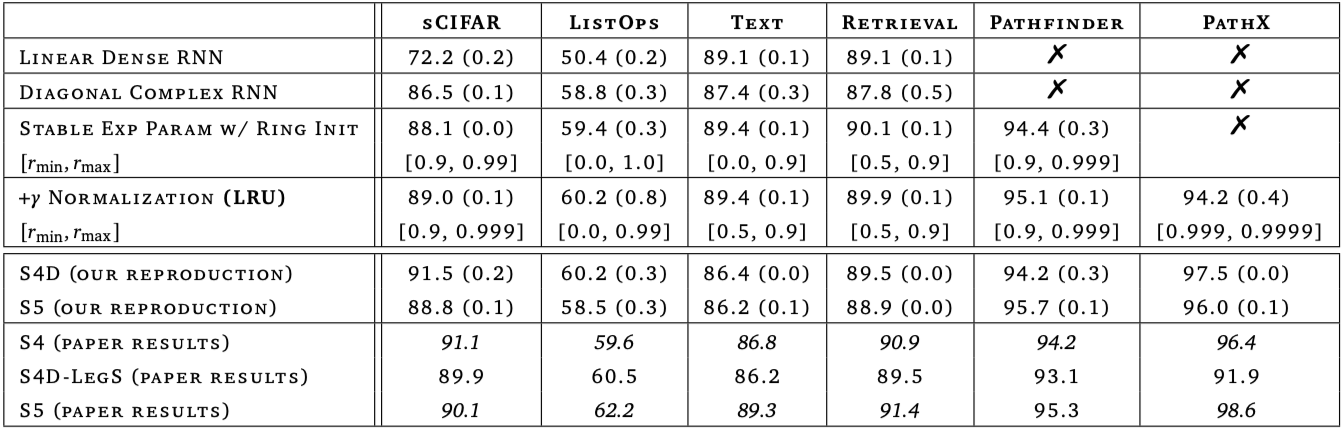
\includegraphics[scale=0.65]{C5.2.4_LRU_Perf.png}}
    \caption{Effects of normalization on linear diagonal RNNs with stable exponential parameterization. Results showcase the advantage of taking initialization close to the unit circle under proper $\mathbf{\gamma}$ normalization.}
    \label{lru-perf}
\end{figure}

With these carefully designed modifications, LRUs achieved impressive performance on the LRA benchmark \cite{lra}, comparable to the S4 Models \cite{s4} as evident from \ref{lru-perf}. LRUs offer a computationally efficient alternative to SSMs and Transformers, especially for tasks requiring the processing of long sequences. Note that for this comparison, they used networks with depth of $6$ residual blocks, with each block consisting of identity skip connection, and the residual path containing a normalization layer\footnote{They used Batch Normalization for all}, followed by the RNN/SSM block.

\medskip

LRUs showcase the effectiveness of systematically analyzing and improving traditional RNNs, guided by insights from both theoretical analysis and the success of SSMs. They offer a powerful and computationally efficient alternative to attention, especially for tasks demanding the processing of long sequences.

\chapter{Hybrid Models: Hawk and Griffin}

Building upon the success of LRUs, De et al. \cite{hawkgriffin} introduced Hawk, a pure RNN model, and Griffin, a hybrid model that combines gated linear recurrences with local attention. These models further push the boundaries of efficient long-range sequence modelling, achieving performance comparable to Transformers \cite{transformers} while maintaining linear scaling in sequence length and exhibiting faster inference speeds.

\section{Model Architecture with Residual Blocks}

\begin{figure}[ht]
    \centerline{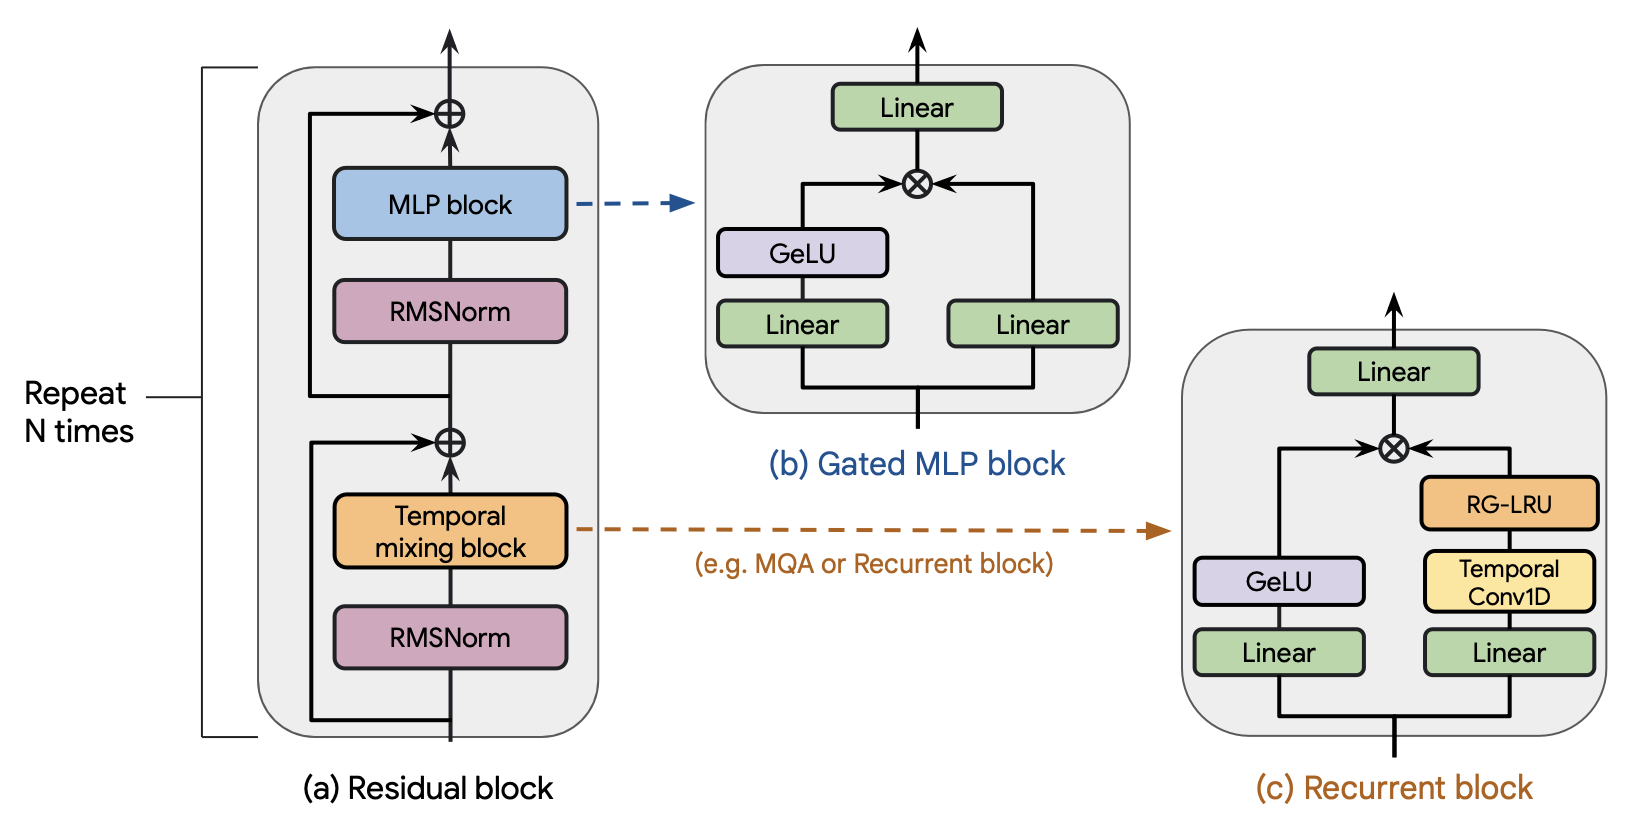
\includegraphics[scale=0.4]{C5.3.1_ResBlock_Arch.png}}
    \caption{(a) The main backbone of Hawk and Griffin is the residual block, which is stacked $N$ times. (b) The gated MLP Block (c) The Recurrent Block containing the RG-LRU layer. For baseline comparison, this recurrent block is replaced with Multi-Query Attention (MQA) \cite{mqa}.}
    \label{hg_resblock_arch}
\end{figure}

Both Hawk and Griffin adopt a similar architecture to Transformers and deep LRUs, employing residual blocks as their main building blocks. These residual blocks, shown in \ref{hg_resblock_arch}(a) of the Griffin paper \cite{hawkgriffin}, consist of:
\begin{itemize}
    \item \textbf{RMSNorm}: Instead of Layer Normalisation, Hawk and Griffin utilize Root Mean Square Layer Normalization (RMSNorm) by Zhang et al. \cite{llama}, which has been empirically beneficial for Transformer-based language models.
    \item \textbf{Temporal Mixing Block}: As illustrated in \ref{hg_resblock_arch}(c), this is the core component that distinguishes Hawk and Griffin. They replace the MQA/MHA block in Transformers with either a recurrent block (for Hawk) or a combination of recurrent and local attention blocks (for Griffin).
    \item \textbf{Gated MLP Block}: Similar to Transformers, a gated MLP block is applied to each token's representation after the temporal mixing block. The details of this block are illustrated in \ref{hg_resblock_arch}(b).
\end{itemize}

\section{RG-LRU: A Modification of LRU}

The recurrent block in Hawk and Griffin employs a modified version of the LRU, called the Real-Gated Linear Recurrent Unit (RG-LRU). This modification introduces gating mechanisms to the LRU, enhancing its ability to selectively propagate or forget information based on the input. The RG-LRU equations are as follows:
\[
\begin{aligned}
\mathbf{r}_t &= \sigma(\mathbf{W}_a \mathbf{x}_t + \mathbf{b}_a), \text{ recurrence gate}\\
\mathbf{i}_t &= \sigma(\mathbf{W}_x \mathbf{x}_t + \mathbf{b}_x), \text{ input gate} \\
\mathbf{a}_t &= \mathbf{a}^{c \mathbf{r}_t}, \\
\mathbf{h}_t &= \mathbf{a}_t \odot \mathbf{h}_{t-1} + \sqrt{1 - \mathbf{a}_t^2} \odot (\mathbf{i}_t \odot \mathbf{x}_t).
\end{aligned}
\]

The output of the layer is $\mathbf{y}_t = \mathbf{h}_t$, and the sigmoid function is denoted by $\sigma$. The recurrent weight $\mathbf{a}$ is diagonal, allowing for element-wise operations. To ensure stability, $\mathbf{a}$ is parameterized as $\mathbf{a} = \sigma(\mathbf{\Lambda})$, where $\mathbf{\Lambda}$ is a learnable parameter, and $c$ is a scalar constant set to $8$.

\subsection{Gating mechanism of RG-LRU}
The input gate, $\mathbf{i}_t$, is similar to that in LSTMs, which allows filtering (scaling down) the input $\mathbf{x}_t$. The recurrence gate, $\mathbf{r}_t$, is unique to the RG-LRU. While the selection mechanism in Mamba \cite{mamba} interpolates between the previous hidden state and the current input, similar to the update gate in GRUs, the recurrence gate in RG-LRU can approximately interpolate between the standard LRU update and the previous state. This allows it to discard the input effectively and preserve information from the previous history. This capability is crucial for achieving super-exponential memory by reducing the influence of uninformative inputs.

\subsection{Temporal Conv 1D Layer}

Unlike the LRU, the RG-LRU layer incorporates a small depthwise 1D convolutional layer before the recurrence. This convolutional layer, inspired by the Shift-SSM in H3 \cite{h3}, operates on a short temporal context (filter dimension of 4). It provides local context to the RG-LRU layer, enhancing its ability to capture short-term dependencies. The output of the convolutional layer is then fed into the RG-LRU layer, as illustrated in \ref{hg_resblock_arch}(c).

\section{Local Sliding Window Attention}
Griffin utilizes local attention, also known as sliding window attention, to further improve its ability to model sequences. This local attention mechanism allows each token to attend only to a fixed number of tokens within a local window, reducing computational complexity compared to global attention while still capturing relevant contextual information. The combination of local attention with the global receptive field of the RG-LRU provides a powerful and efficient mechanism for sequence modelling.

\section{Hawk}
Hawk is a pure RNN model that solely relies on RG-LRU blocks for temporal mixing. Its architecture comprises stacking multiple residual blocks, each containing an RG-LRU layer followed by a gated MLP block and residual connections.

\section{Griffin}
Griffin combines the strengths of RG-LRU and local attention. Its architecture alternates between two residual blocks with an RG-LRU layer and one residual block with a local sliding window attention layer. This layered structure enables Griffin to capture both long-range dependencies (through RG-LRU) and local context (through local attention), leading to improved performance and efficiency.

\section{Optimisations}
To further enhance computational efficiency, especially on modern hardware, Griffin incorporates a custom linear scan implementation for the RG-LRU layer (similar to Mamba \cite{mamba}). This optimisation is crucial because diagonal RNNs, like RG-LRU, have a low FLOPs-to-byte ratio, making them memory-bound on current accelerators. The custom linear scan minimises memory transfers by keeping the hidden state in the fast on-chip memory (SRAM) throughout the computation.

\section{Empirical Results}
Both Hawk and Griffin have achieved remarkable results on language modelling tasks, showcasing their potential as efficient alternatives to Transformers:

\subsection{Scaling Laws and Throughput}

\begin{figure}[ht]
    \centerline{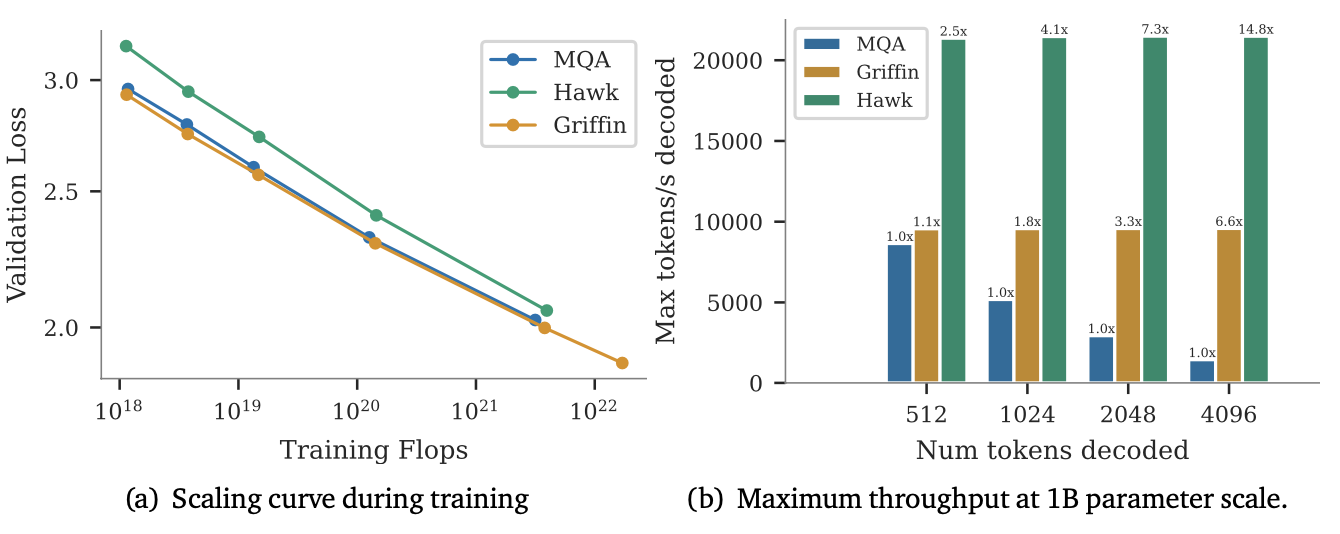
\includegraphics[scale=0.6]{C5.3.7_Griffin_Scaling.png}}
    \caption{Comparing validation loss and throughput of Hawk, Griffin and MQA on custom dataset.}
    \label{hg_scaling}
\end{figure}

As evident from \ref{hg_scaling}(a), Hawk, Griffin and MQA baseline exhibit power law scaling between validation loss and training FLOPs, with Griffin achieving the lowest validation loss. In terms of throughput, both Griffin and Hawk thoroughly outperform MQA, especially as the length of the sample increases, as shown in \ref{hg_scaling}(b).


\subsection{Character Normalised Accuracy}

\begin{figure}[ht]
    \centerline{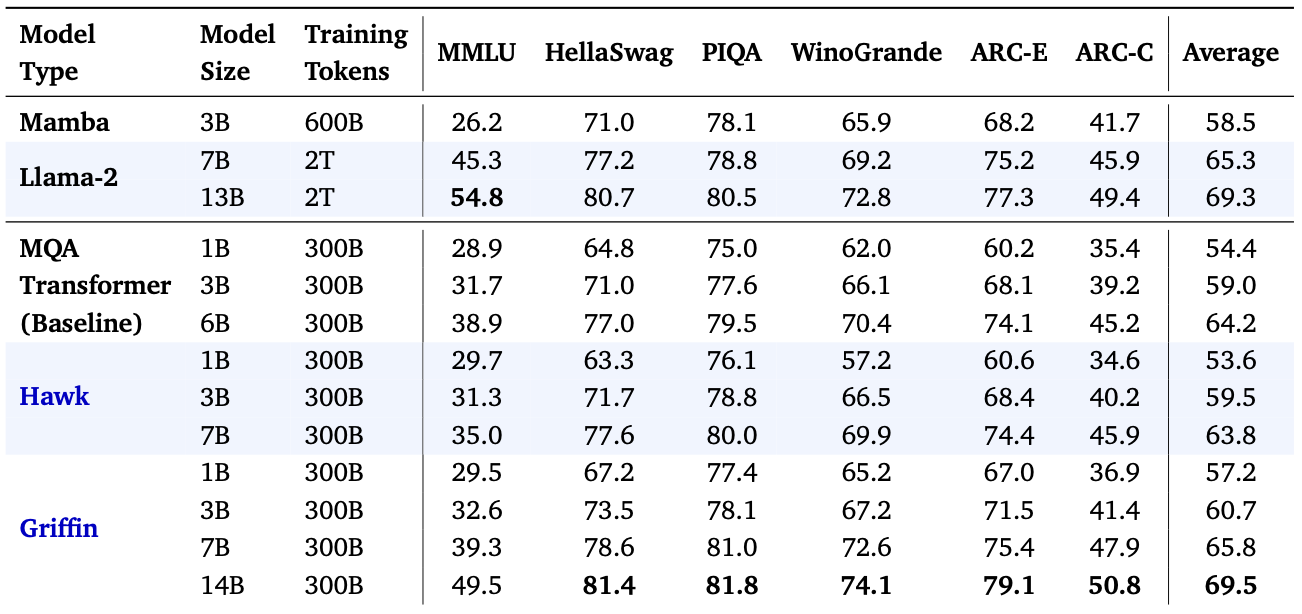
\includegraphics[scale=0.65]{C5.3.7_Griffin_Perf.png}}
    \caption{Comparison of character normalized accuracy of different models of different sizes on various downstream tasks.}
    \label{griffin-perf}
\end{figure}

As shown by this table at \ref{griffin-perf}, the character-normalised accuracy of Hawk and Griffin on various downstream tasks. Hawk exceeds the performance of Mamba \cite{mamba}, while Griffin achieves comparable accuracy to LLaMA-2 \cite{llama2}, despite being trained on significantly fewer tokens. Note that the pre-training datasets used here are different.

\medskip

These results, combined with their efficiency advantages in training and inference, position Hawk and Griffin as compelling alternatives to attention-based models.

\chapter{Experiments}

In this chapter, we present some results from the experiments conducted using the Transformer and Mamba models on three different datasets: Tiny Shakespeare, Maestro V2, and Sequential MNIST. The experiments aimed to compare the performance of the two models on diverse tasks, including character-level language modelling, MIDI generation, and sequential digit generation.

\medskip

Here is a brief over of the models used in the experiments:
\begin{itemize}
    \item \textbf{Transformer}: The Transformer model used in the experiments is based on GPT-2 architecture \cite{gpt2}, inspired by the nanoGPT repository by Andrej Karpathy. It consists of a stack of Decoder Blocks, each containing a Multi-Head Self-Attention layer and a MLP layer. Due to limited compute, we stuck to a smaller model with $2.4M$ parameters. We fix a cosine decay learning rate schedule, starting from $10^{-3}$ and decaying to $10^{-4}$ over the course of training.
    \item \textbf{Mamba}: Due to limited resources, we used a smaller model with $2.2M$ parameters for Mamba as well. For Mamba we use $10$ times smaller learning rate than the Transformer model. So, we use a cosine decay learning rate schedule, starting from $10^{-4}$ and decaying to $10^{-5}$ over the course of training.
\end{itemize}

Note, we could not experiment with Hawk and Griffin, as they require more modern GPUs supporting newer versions of Triton.

\section{Tiny Shakespeare}

The Tiny Shakespeare dataset \cite{tinyshakespeare} consists of 40,000 lines of text from various plays by William Shakespeare. The task is to train a character-level language model to generate text similar to Shakespeare's writing style. Here, we use a vocabulary of $65$ characters and a context length of $256$ tokens.

\begin{figure}[ht]
    \centering
    \begin{minipage}[b]{0.45\textwidth}
        \centering
        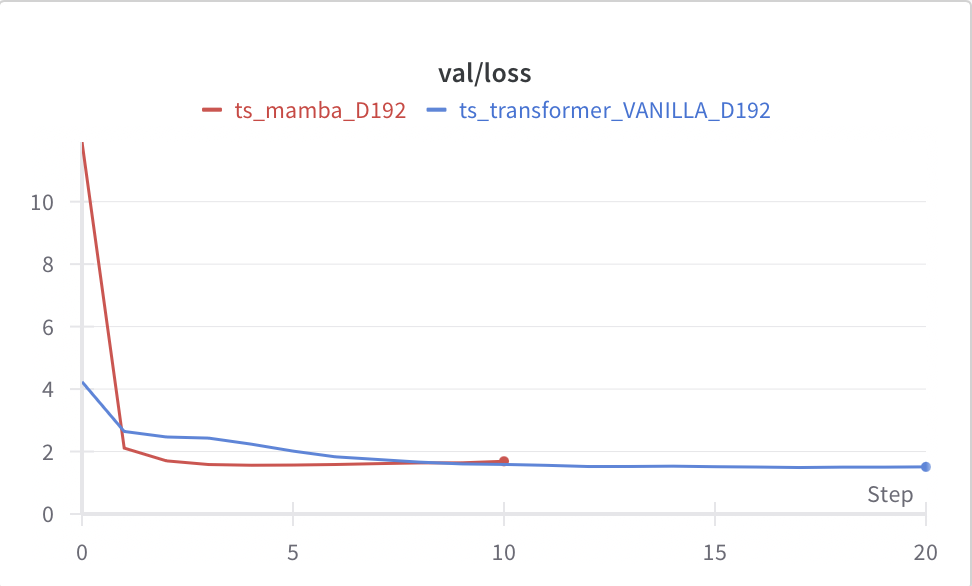
\includegraphics[scale=0.4]{experiments/ts/ts_loss.png}
        \caption{Tiny Shakespeare: Loss Curves}
        \label{ts-loss}
    \end{minipage}
    \hspace{0.05\textwidth}
    \begin{minipage}[b]{0.45\textwidth}
        \centering
        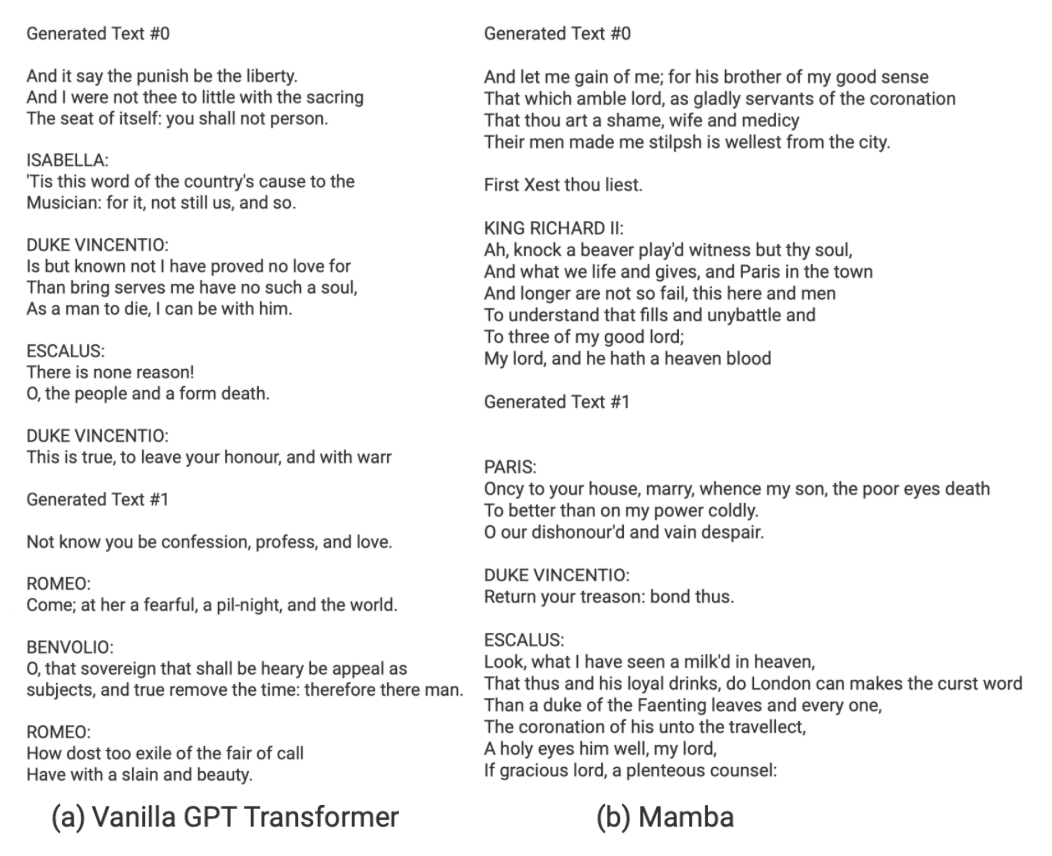
\includegraphics[scale=0.4]{experiments/ts/ts_gen.png}
        \caption{Generated text samples}
        \label{ts-gen}
    \end{minipage}
\end{figure}

As evident from \ref{ts-loss}, Mamba seems to converge faster than the Transformer model, even though it has a lower learning rate, but it ends up overfitting the data. The generated text samples in \ref{ts-gen} show that both models are able to generate text that resembles Shakespeare's writing style from scratch.

\section{Maestro V2}

The Maestro V2 dataset \cite{maestrov2} contains about 200 hours of paired audio and MIDI recordings from ten years of International Piano-e-Competition. The task is to train a MIDI generating model that can generate music similar to the pieces in the dataset. We first preprocess the MIDI files using the MidiTok library to tokenize the MIDI files using a BPE tokenizer. Here, we use a vocabulary of $8000$ tokens and a context length of $256$ tokens.

\begin{figure}[ht]
    \centerline{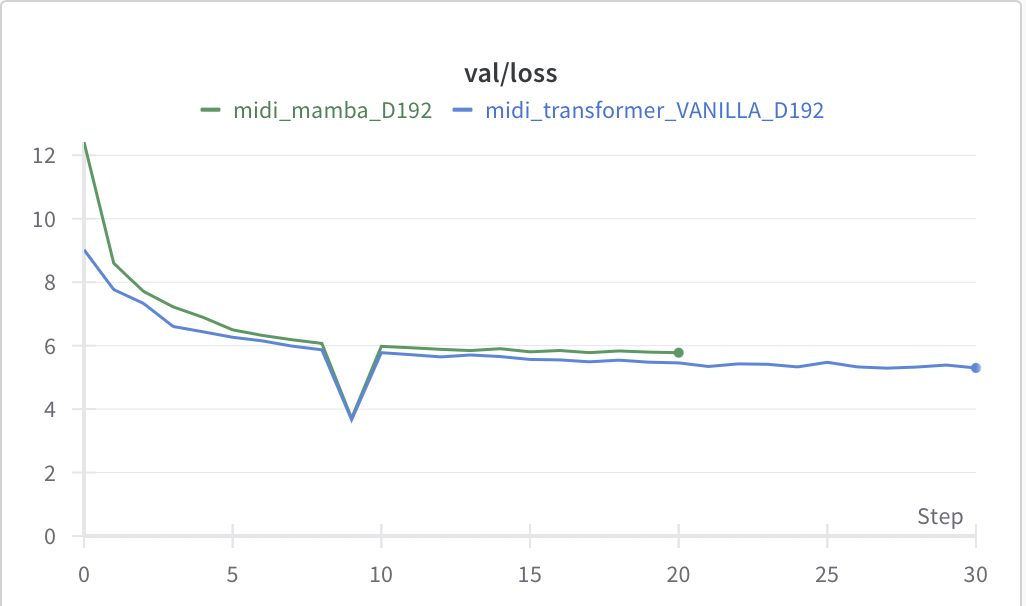
\includegraphics[scale=0.45]{experiments/midi/midi_loss.png}}
    \caption{MIDI: Loss Curves}
    \label{midi-loss}
\end{figure}

Repeating the trend, Mamba converges faster than the Transformer model, as seen in \ref{midi-loss}, even though it has a lower learning rate. But it still ends up overfitting the data. The generated MIDI samples from both models are not shown here, but they are available in the code repository.

\section{Sequential MNIST}

The Sequential MNIST dataset is a modified version of the MNIST dataset \cite{mnist}, where we quantize the pixel values to $3$-bit pixels with values from $[0, 7]$. We reshape the $28 \times 28$ images to $16 \times 16$ and flatten them to a $256$-dimensional array. We can flatten the images using various strategies, but from empirical observations the best results were obtained using the identity flattening strategy, where we flatten the image from left to right, one row after another. We train our models only on the digit $0$ to make the task easier and converge faster.

\begin{figure}[ht]
    \centering
    \begin{minipage}[b]{0.45\textwidth}
        \centering
        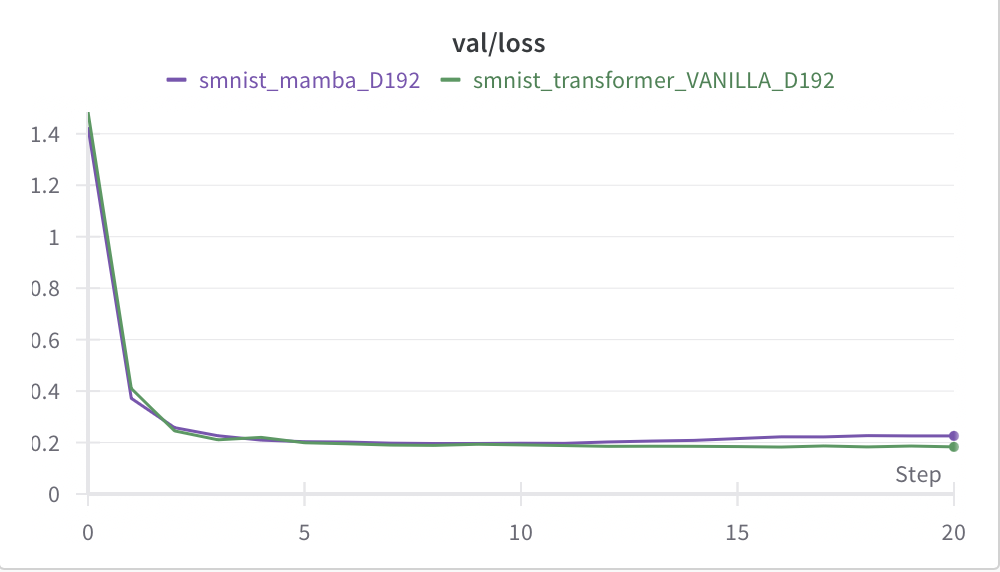
\includegraphics[scale=0.4]{experiments/smnist/smnist_final_loss.png}
        \caption{SMNIST: Loss Curves}
        \label{smnist-loss}
    \end{minipage}
    \hspace{0.05\textwidth}
    \begin{minipage}[b]{0.45\textwidth}
        \centering
        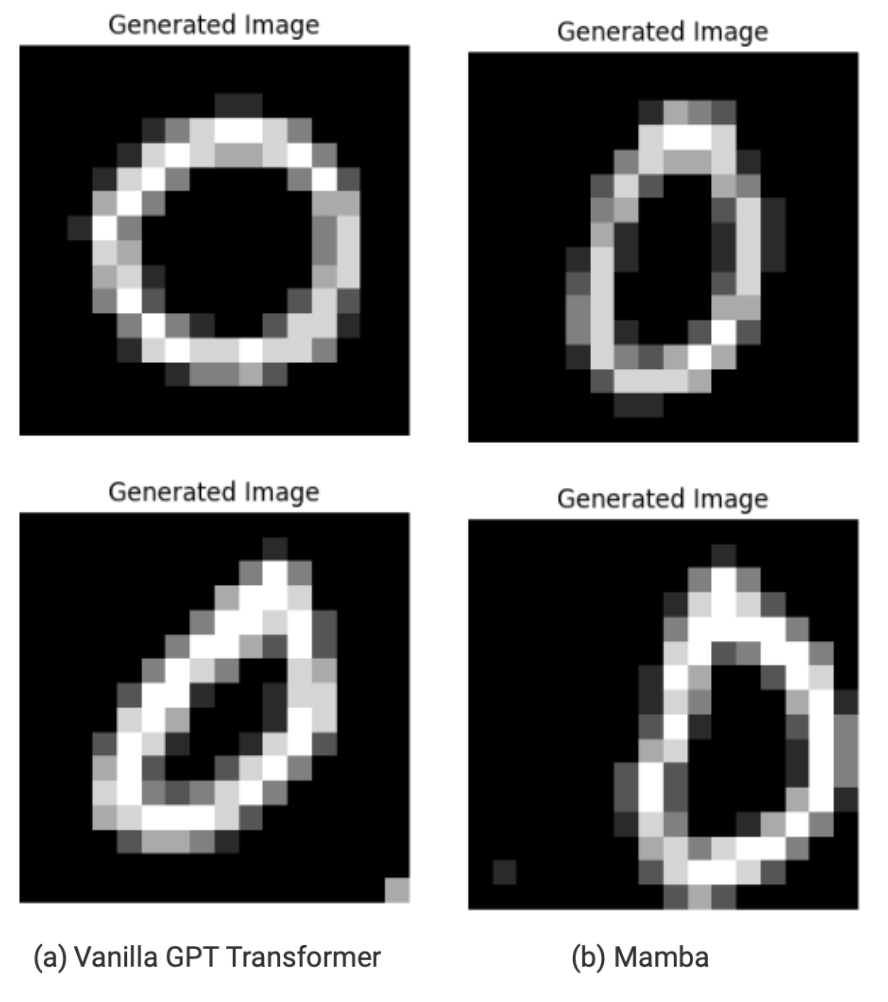
\includegraphics[scale=0.3]{experiments/smnist/smnist_gen.png}
        \caption{Generated digit samples}
        \label{smnist-gen}
    \end{minipage}
\end{figure}

As seen in \ref{smnist-loss}, Mamba ends up slightly overfitting on the data again. The generated digit samples from both the models are shown in \ref{smnist-gen}. Both models are able to sequentially generate digits pixel-by-pixel from scratch.

% Bibliography
\printbibliography

\end{document}